\documentclass[a4paper, 12pt]{book}

\usepackage[utf8]{inputenc}
\usepackage{lmodern}
\usepackage{enumitem}
\usepackage{layout}
\usepackage{emptypage}
\usepackage{fancyhdr}
\usepackage{fancyref}
\usepackage{fancyvrb}
\usepackage{subcaption} % subfiguras
\usepackage{caption}
\usepackage{mathtools}
\usepackage{hyperref}
\usepackage[a4paper,top=3cm, bottom=3cm, inner=2.5cm, outer=2.5cm]{geometry}
\usepackage{listings}
\usepackage[english]{babel}
\usepackage{url}
\usepackage{color}
\usepackage[normalem]{ulem}
\usepackage[dvipsnames]{xcolor}
\usepackage{biblatex}\addbibresource{Bibliography.bib}
\usepackage{amsmath}
\usepackage{algorithm}
\usepackage{amsmath}
\usepackage[noend]{algpseudocode}
\usepackage[nottoc,numbib]{tocbibind}
\usepackage{mathtools}
\usepackage{graphicx}
\newcommand*{\matminus}{%
	\leavevmode
	\hphantom{0}%
	\llap{%
		\settowidth{\dimen0 }{$0$}%
		\resizebox{1.1\dimen0 }{\height}{$-$}%
	}%
}
\definecolor{codegreen}{rgb}{0,0.6,0}
\definecolor{codegray}{rgb}{0.5,0.5,0.5}
\definecolor{codepurple}{rgb}{0.58,0,0.82}
\definecolor{backcolour}{rgb}{0.95,0.95,0.92}

\lstset{frame=single,
	language=Python,
	aboveskip=3mm,
	belowskip=3mm,
	showstringspaces=false,
	columns=flexible,
	basicstyle={\small\ttfamily},
	numbers=none,
	backgroundcolor=\color{backcolour},   
	commentstyle=\color{codegreen},
	keywordstyle=\color{blue},
	numberstyle=\color{codepurple},
	stringstyle=\color{magenta},
	breaklines=true,
	breakatwhitespace=true,
	tabsize=3
}

\newcommand{\etal}{\textit{et al}. }
\newcommand{\ie}{\textit{i}.\textit{e}., }
\newcommand{\eg}{\textit{e}.\textit{g}. }

\usepackage[acronym,nomain]{glossaries}
\newacronym{ml}{ML}{Machine Learning}
\newacronym{dl}{DL}{Deep Learning}
\newacronym{cnn}{CNN}{Convolutional Neural Network}
\newacronym{nn}{NN}{Neural Network}
\newacronym{cpm}{CPM}{Convolutional Pose Machines}
\makeglossaries

%\usepackage{titlesec}
\makeatletter
\renewcommand{\@makeschapterhead}[1]{
  \vspace*{0\p@}%
  {\parindent \z@ \raggedright
    \normalfont
    \interlinepenalty\@M
    \Huge \bfseries  #1\par \nobreak
    \vskip 15\p@
  }}
\makeatother

\renewcommand{\baselinestretch}{1.4}
\setlength{\headheight}{16pt} 

\pretolerance=1000

\chead[]{}
\rhead[]{}
\renewcommand{\headrulewidth}{0.5pt}

\pagestyle{empty}

\title{3D Human Pose Estimation for Assistive Robotics}
\author{David Pascual Hernández}

\begin{document}
%%%%%%%%%%%%%%% Cover %%%%%%%%%%%%%%%%%%%%
\begin{titlepage}
	\begin{center}
		\vspace*{7.7mm}
		\begin{center}
			
\includegraphics[width=0.4\linewidth]{figures/logo.jpg}
		\end{center}
		\vspace{6.5mm}
		
		\fontsize{14}{14}\selectfont MÁSTER UNIVERSITARIO \\ EN VISIÓN ARTIFICIAL

		\vspace{70pt}
		
		\fontfamily{lmss}\fontsize{15.7}{14}\selectfont \textbf{TRABAJO FIN DE MÁSTER} 
		
		\vspace{25mm}
		\begin{huge}
    		Real-time 3D Human Pose Estimation
    		\vspace{1cm}
    		for Robotics Applications
		\end{huge}
		
		\vspace{25mm}
		
		\begin{large}
			Autor: David Pascual Hernández
			
			Tutor: José María Cañas Plaza
			
			Co-tutora: Inmaculada Mora Jiménez 
			
			\vspace{10mm}
		\end{large}
		\begin{normalsize}
			Curso académico 2019/2020
		\end{normalsize}
		\vspace{10mm}
		
	\end{center}
	
\end{titlepage}

\pagebreak
\thispagestyle{empty}
\vspace*{12cm}

\begin{flushright}
	
	
\includegraphics[height=1.0cm]{figures/CC-BY-SA.png}
	
	\vspace*{0.5cm}
	
	\copyright 2020 David Pascual Hernández
	
	\vspace*{0.3cm}
	
	Esta obra está distribuida bajo la licencia de 
	
	``Reconocimiento-CompartirIgual 4.0 Internacional (CC BY-SA 4.0)''
	
	de Creative Commons.
	
	\vspace{0.2cm}
	
	Para ver una copia de esta licencia, visite
	
	http://creativecommons.org/licenses/by-sa/4.0/ o envíe
	
	una carta a Creative Commons, 171 Second Street, Suite 300,
	
	San Francisco, California 94105, USA.
	
\end{flushright}


\pagebreak
\thispagestyle{empty}
\vspace*{12cm}

\begin{flushright}
	
RoboCity2030 - Madrid Robotics Digital Innovation Hub

Programa de Actividades de I+D entre Grupos de investigación de la

Comunidad de Madrid en Tecnologías 2018, Comunidad de Madrid.

Ref S2018/NMT-4331

Acrónimo: RoboCity2030-DIH-CM

\vspace{1cm}

\emph{This work has been partly supported by the Spanish}

\emph{Ministry of Economy under the grants with reference}

\emph{TEC2016-75361-R and PID2019-106623RB-C41.}

\end{flushright}

\pagenumbering{Roman}

%%%%%%%%%%%%%%% Acknowledgements %%%%%%%%%%%%
%\chapter*{}
%\pagenumbering{Roman} % para comenzar la numeracion de paginas en numeros romanos
%\begin{flushright}
%	\textit{``I'm afraid that the following syllogism may be used by some in the future:\\	Turing believes machines think.\\	Turing lies with men.\\	Therefore machines do not think."\\  —Alan Turing, 1952}
%\end{flushright}

\chapter*{Agradecimientos}

%%%%%%%%%%%%%%% Resumen %%%%%%%%%%%%%%%%%%%%
\chapter*{Resumen}

%%%%%%%%%%%%%%% Summary %%%%%%%%%%%%%%%%%%%%
\chapter*{Summary}

%%%%%%%%%%%%%%% Índices %%%%%%%%%%%%%%%%%%%%
\tableofcontents
\listoffigures % Í­ndice de figura
\listoftables
\printglossaries
\addcontentsline{toc}{chapter}{Acronyms}
\cleardoublepage

%%%%%%%%%%%%%%% Chapters %%%%%%%%%%%%%%%%%%
\pagestyle{fancy}
\pagenumbering{arabic}
\setlength{\parindent}{6mm}

\lhead[]{CHAPTER \thechapter. INTRODUCTION}
\chapter{Introduction}\label{ch:introduction}
\lhead[]{CHAPTER \thechapter. RELATED WORK}
\chapter{Related Work}\label{ch:related_work}
\lhead[]{CHAPTER \thechapter. DIGIT CLASSIFIER}
\chapter{Proposed method}\label{ch:proposed_method}
As we pointed out in the previous chapter, human pose estimation is a problem that can be approached from a multitude of different perspectives. After extensively reviewing previous work in the field, and taking into account the particular requirements of robotics applications, we propose a very lightweight solution for 3D estimation from RGBD data that builds upon some of the methods presented in Section~\ref{subsec:dl_2d_estimation}. In this chapter, we present an overview of our system and its components. We have split our process into two major blocks: 2D and 3D estimation. For the former, three 2D human pose estimators have been tested. First, their architectures and training strategies are described and their pros and cons are discussed. Then, our method for getting 3D estimations from 2D coordinates is presented with greater detail, showing how each individual step works and how they contribute to the overall system performance. 

\section{System design}
As previously stated in Section~\ref{sec:goals}, our main objective is to build a system for 3D human pose estimation that is lightweight enough to be embedded in a robot and that can operate independently of the point of view, while perceiving in real-time the poses of the humans around. Keeping these requirements in mind, we have decided to design a hybrid system that relies on \gls{sota} \gls{dl}-based solutions for 2D human pose estimation and a very straight-forward method for augmenting the estimated 2D keypoints to 3D, leveraging the depth information provided by an RGBD sensor. An overview of this system is shown in Figure~\ref{fig:system_design}.

\begin{figure}[h]
    \centering
    \includesvg[width=\textwidth]{figures/system_design_v02.svg}
    \caption{Overview of the pipeline proposed for 3D human pose estimation.}
    \label{fig:system_design}
\end{figure}

Our method does not make any assumption on the kind of algorithm used for estimating the 2D coordinates, and so one can choose the 2D human pose estimator that better fits the particular application being developed. This flexibility allows the user to prioritize accuracy over computational cost or vice versa. It also ensures that our pipeline can be updated with novel solutions for 2D pose estimation that might be proposed in the years to come. It is important to mention that human detection is a required step before most of the available 2D pose estimators in the literature, but this step is out of the scope of this work, as there are some methods that might perform human and pose detection jointly~\cite{cao2018openpose}. For completeness, we will present a briefly description of how we achieve human detection in the next section, without going into great detail.

Regarding the 2D to 3D estimation step, we will assume that a commercial RGBD sensor is available. This is a reasonable assumption taking into account how widespread and affordable some of these sensors have become in the last years. Such is the case of the \emph{Asus Xtion} sensor~\cite{xtion}, which we will use to experimentally validate our system in Section~\ref{sec:demo}. Our proposed method for estimating the 3D coordinates from the detected 2D keypoints relies on classic computer vision techniques that are well established and that fulfill our requirements in terms of computational costs. Furthermore, the only specific step for human pose estimation in this method is the outlier rejection, and so it can be easily adapted for any kind of 3D estimation given its 2D counterparts.

\section{2D Estimation}\label{sec:2d_estimation}
In order to estimate the initial 2D locations of the human joints considered, we have evaluated the usage of three different \gls{dl}-based solutions, which have provided good results in the literature. None of them make use of explicit graphical models. The tested methods have been chosen both for their performance, in terms of the leap forward they represented for the human pose estimation field, and their intuitiveness, which will be useful to ensure a clear analysis of the results obtained. Before presenting these methods, we will start by addressing how human detection can be performed for further improving the pose estimation results.

\subsubsection{Human detection}\label{subsubsec:human_detection}
Human detection is a well studied area of computer vision, which can be considered a subfield of the more generic object detection problem. Detecting humans in 2D images is specially challenging due to the variable appearance a human body can take when projected in a 2D surface, which is highly dependent on properties like pose and clothing. We are not going to dive deep into human detection literature, but it is worth mentioning the classic approach proposed by Dalal and Triggs~\cite{dalal2005histograms}, as it is probably one of the most relevant works in the field. In their work, they build a grid of \emph{Histograms of Oriented Gradients} and classify the resulting patches using \emph{Support Vector Machines}. This is a very efficient method and, for years, it has been established as the go-to solution for human detection.

However, as it has happened for most of the classic problems in computer vision, \gls{dl} solutions have demonstrated to be far more accurate. This is specially true in the case of human detection, as there is huge availability of potential training data. Taking that into account, we have used an \emph{SSDLite MobileNetV2} model as our baseline human detector~\cite{sandler2018mobilenetv2}. It is not only precise enough for our application, but it also has been specifically built to be as lightweight as possible to ensure it is suitable for being embedded in systems with scarce resources, hence the \emph{mobile} prefix in its name. This model is based on the successful \emph{Single Shot Multibox Detector}, initially introduced by Liu \etal\cite{liu2016ssd} (see Figure~\ref{fig:ssd}), but tweaked with a novel layer that uses depth-wise separable convolutions to improve the efficiency of the model by reducing the number of parameters and operations needed during inference. The trained model is publicly available as part of the \emph{TesorFlow Model Garden}~\footnote{\url{https://github.com/tensorflow/models/tree/master/research/slim/nets/mobilenet}}.

\begin{figure}[h]
    \centering
    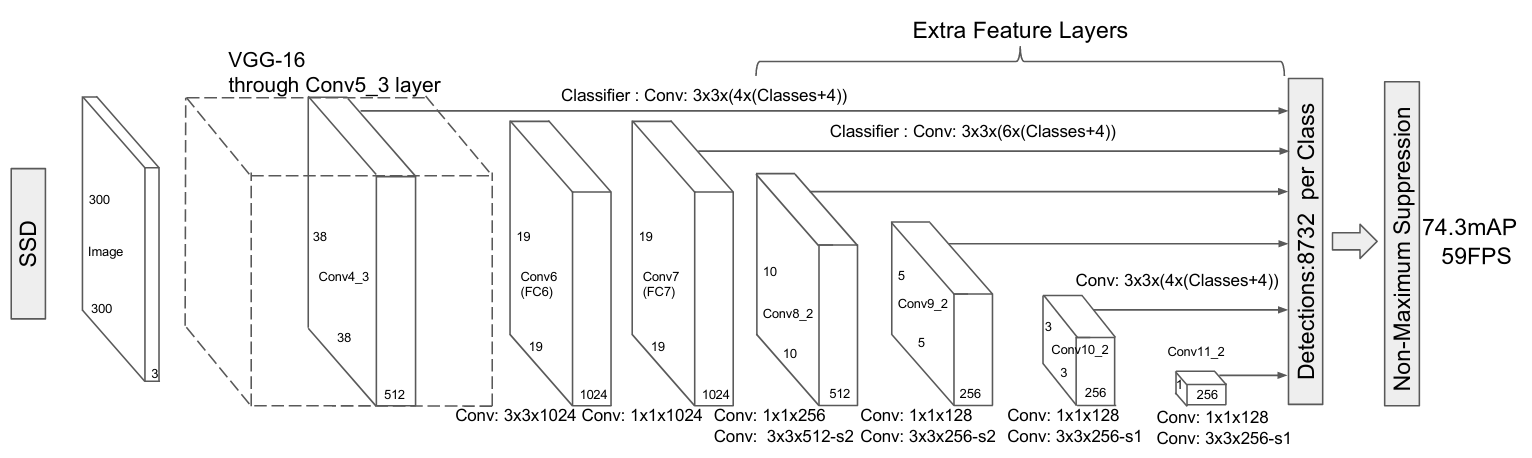
\includegraphics[width=\textwidth]{figures/ssd.png}
    \caption{\emph{Single Shot Multibox Detector} architecture as presented by Liu \etal\cite{liu2016ssd}. In the \emph{SSDLite MobileNetV2} adaptation, the convolutional layers are replaced by the depth-wise separable convolutions proposed in ~\cite{sandler2018mobilenetv2}.}
    \label{fig:ssd}
\end{figure}

\subsection{Convolutional Pose Machines}\label{subsec:cmps}
\glspl{cpm}, introduced by Wei \etal in~\cite{Wei2016-rb}, is one of the most prominent works in the 2D human pose estimation field, as it laid the foundation for the \emph{OpenPose} suite (see Section~\ref{subsec:dl_2d_estimation}). Broadly speaking, the architecture proposed by Wei \etal is a combination of multi-class predictors organized into several stages. Each of these multi-class predictors is built as a \gls{cnn} estimating the location of a single human joint. The image features and belief maps produced by each of these predictors in one stage are used as input for the next one. With each subsequent stage, the receptive field over the input image increases, implicitly encoding contextual information and allowing the network to learn correlations between parts. This effect is well exemplified in Figure~\ref{fig:cpms}, which summarizes the \glspl{cpm} architecture and shows the receptive field at different stages for an example image. In the original article, results are reported for a \gls{cpm} composed of 6 stages.

\begin{figure}[h]
    \centering
    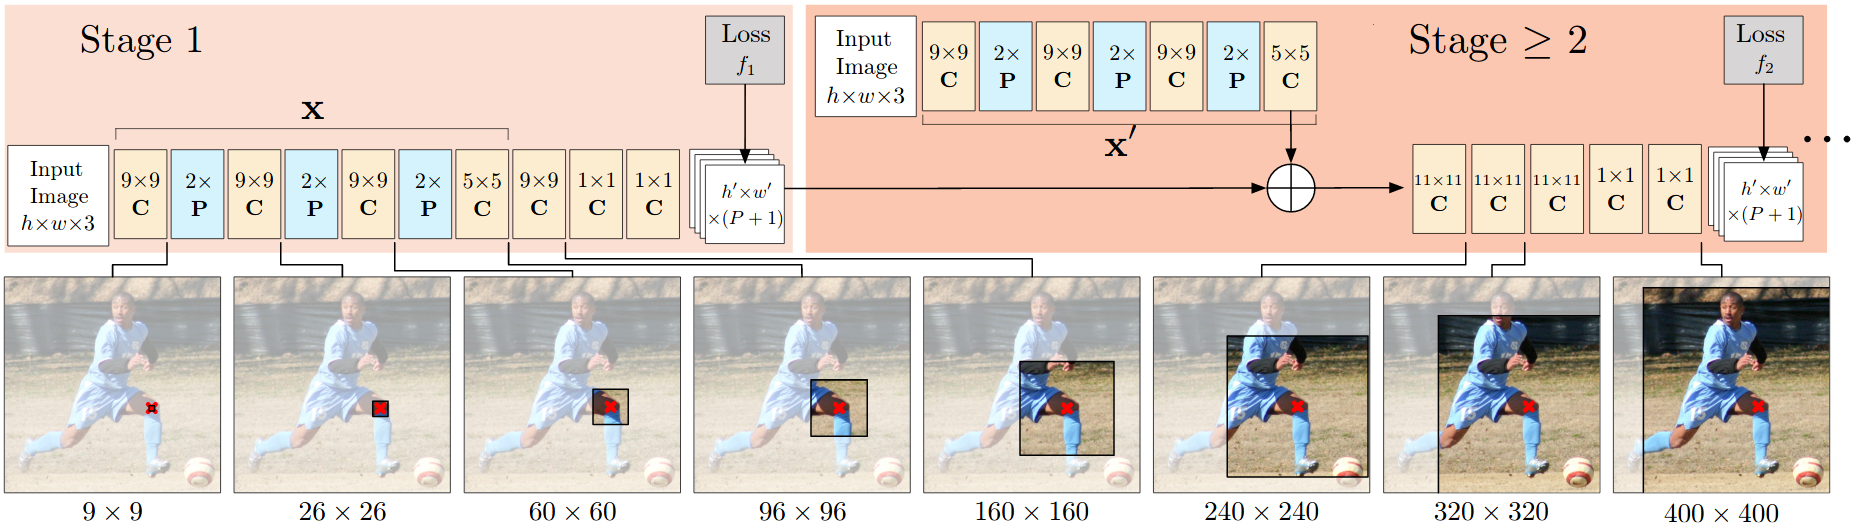
\includegraphics[width=\textwidth]{figures/cpms.png}
    \caption{Overview of the CPMs model proposed by Wei \etal\cite{Wei2016-rb}. The top of the diagram shows the architecture of the first stage and the subsequent ones. In the bottom, the increment in the receptive field across each new stage is shown.}
    \label{fig:cpms}
\end{figure}

Regarding the model training, each stage and body part has its own specific loss function, computed as the squared error between the predicted and the target belief maps. It is worth clarifying that the target belief map of each body part is created by locating a \emph{Gaussian} function at the ground-truth location. The individual losses that we have just described are then aggregated to provide the overall loss of the \gls{cpm} being trained. In that way, all the weights involved in each of the stages and predictors can be jointly trained with intermediate supervision. During evaluation, input images are cropped in a square around the subject of interest and normalized to a size of 368x368 pixels.

\subsection{Stacked Hourglass}\label{subsec:sh}
Newell \etal\cite{Newell2016-cy} propose a novel \gls{cnn} architecture, which leverage features in the image at different scales by repeated \emph{bottom-up} and \emph{top-down} processing steps, \ie from high to low resolution and vice versa, respectively. Each of these \emph{bottom-up} and \emph{top-down} blocks are given the name of \emph{Hourglass Modules}. For the \emph{bottom-up} stage, the images are downsampled by stacking several convolutional and \emph{Max Pooling} layers. For the \emph{top-down} stage, the lowest resolution image passes through several \emph{Nearest Neighbors} upsampling layers until the original resolution is reached. Each \emph{Hourglass Module} is symmetrical and the combination of features at different scales is enforced by elementwise additions between maps of equal resolution from the \emph{top-down} and \emph{bottom-up} halfs of the module. In Figure~\ref{fig:sh}, the architecture of a single \emph{Hourglass Module} is shown in a very intuitive way. In order to further consolidate the multi-scale features extracted by the \gls{cnn} and refine the estimated locations for each joint, several of these modules are stacked together. Newell \etal report their final results for a \gls{sh} model composed of 8 \emph{Hourglass Modules}.

\begin{figure}[h]
    \centering
    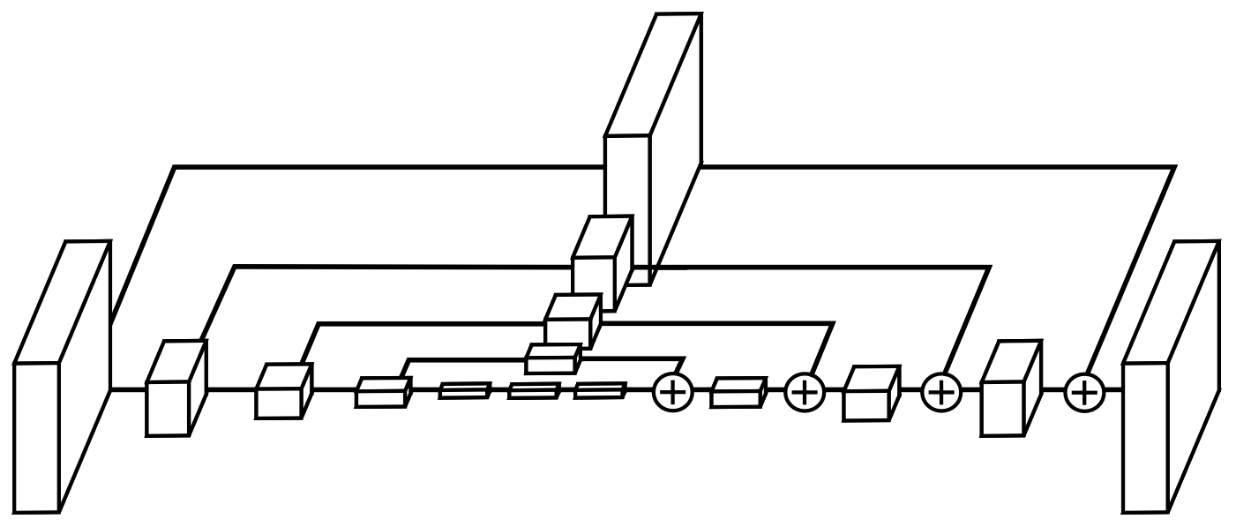
\includegraphics[width=\textwidth]{figures/sh.png}
    \caption{Diagram of a single \emph{Hourglass Module}, the main building block of the \emph{Stacked Hourglass} architecture proposed by Newell \etal\cite{Newell2016-cy}.}
    \label{fig:sh}
\end{figure}

It is worth mentioning that simply stacking \emph{Hourglass Modules} without intermediate supervision would never take the \gls{sh} model to its full potential. This intermediate supervision process is achieved by optimizing the \emph{Mean Squared Error} between the predicted heatmaps and their ground-truth after each module. As in \glspl{cpm}, the target heatmap is created by locating a bi-dimensional \emph{Gaussian} function on each joint location. During evaluation, input samples are cropped and then resized to 256x256 pixels.

\subsection{Chained Predictions}\label{subsec:cp}
The method proposed by Gkioxari \etal\cite{Gkioxari2016-ix} is based on \emph{sequence-to-sequence} models~\cite{sutskever2014sequence}, in which multiple output variables are predicted sequentially, \ie the prediction for a given output does not only depends on the input, but also on the previously predicted output variables. They propose an extension of this kind of models for more general structured outputs taking images as input and demonstrate its performance in human pose estimation, which is a clear example of structured prediction. In their model, the prediction for each body joint is dependent on all previously predicted joints, following a fixed ordering, which is determined according to detection rates yielded by an unchained \emph{feed-forward} net. In that way, the easier cases are processed first, while the harder ones take advantage of all the contextual information given by the previous detected joints. In Figure~\ref{subfig:cp_general}, a diagram showing the \glspl{cp} model can be found. Gkioxari \etal architecture is composed of two main blocks, an encoder that processes the input image with several convolutional operations (\gls{cnn}\textsubscript{x}), and a decoder composed of deconvolutional layers (\gls{cnn}\textsubscript{y}). The image encoded by the \gls{cnn}\textsubscript{x} is shared for every joint, while there is a single \gls{cnn}\textsubscript{y} block for each joint, which takes as input the encoded image and predictions from previous joints. The architecture of each of these blocks is presented in Figure~\ref{subfig:cp_particular}.

\begin{figure}[h]\centering
    \begin{subfigure}{0.41\textwidth}\centering
        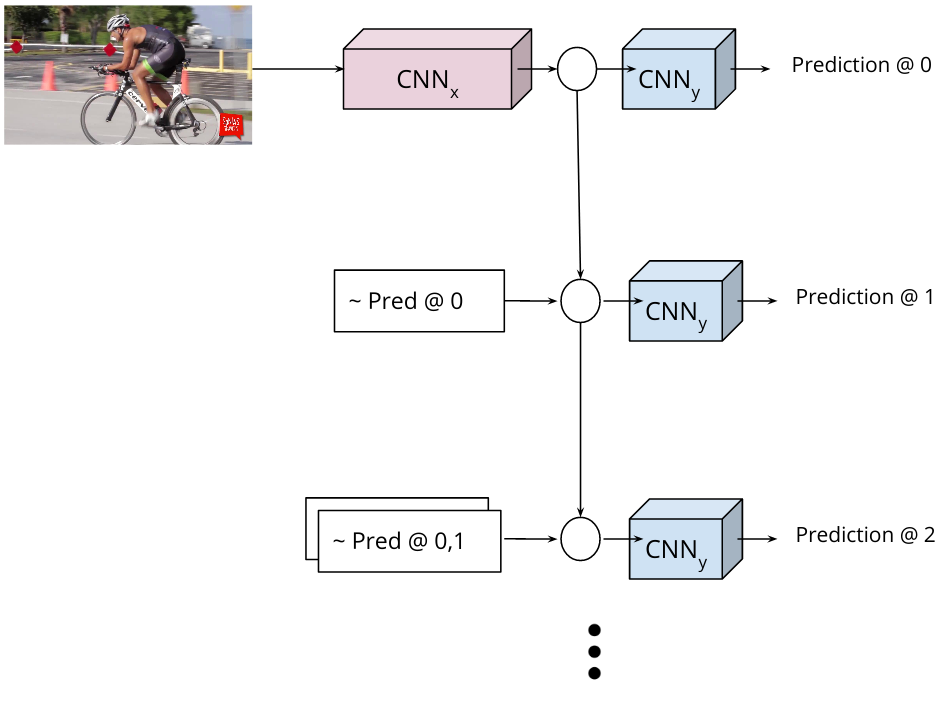
\includegraphics[height=5cm]{figures/cp_general.png} 
        \caption{CPs architecture.}
        \label{subfig:cp_general}
    \end{subfigure}
    \begin{subfigure}{0.58\textwidth}\centering
        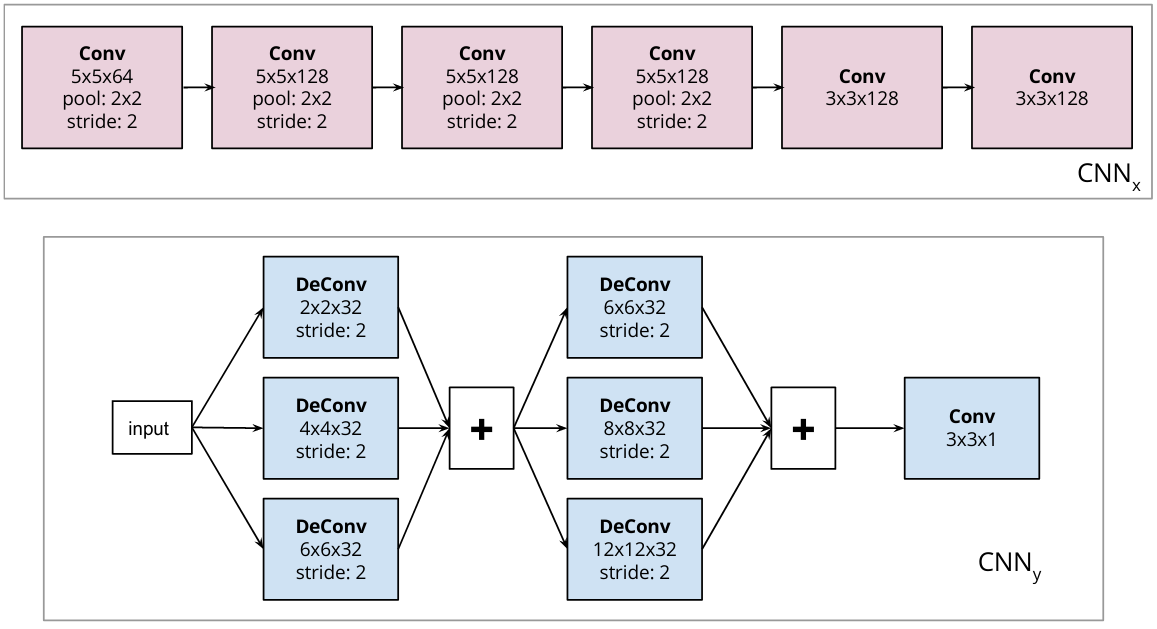
\includegraphics[height=5cm]{figures/cp_particular.png}
        \caption{Main CPs  model blocks.}
        \label{subfig:cp_particular}
    \end{subfigure}
    \caption{In (a), a complete diagram of the CPs architecture proposed by Gkioxari \etal\cite{Gkioxari2016-ix} is shown. The model proposed is composed of a single CNN\textsubscript{x} that encodes the input image, and several CNN\textsubscript{y} (decoders) which, taking as input the encoded image and the previous predictions, return a heatmap for each joint. Both blocks are shown in (b).}
    \label{fig:cp}
\end{figure}

During the first iterations of the training stage, the results from the previous joints predictions are replaced by their ground-truths, as these estimations can be really inaccurate and can jeopardize model convergence. Once the previous predictions start to get better, they are gradually introduced instead of their ground-truths. This training strategy is called \emph{scheduled sampling}, and was initially introduced by Bengio \etal\cite{bengio2015scheduled}. During evaluation, input samples are rescaled to 299x299 pixels.

\subsection{Conceptual comparison}\label{subsec:conceptual_comparison}
As it has been already mentioned, none of these methods are based on an explicit spatial model that takes into account the relation between each joint. Instead, these relations are implicitly learned  during training. In that way, the only model that makes an slight assumption regarding how each joint relates to each other is \glspl{cp}, which have a fixed order for its sequential prediction. However, even in that case, the order is previously decided by the accuracy obtained for each joint when estimating their locations using a \emph{feed-forward} net, so it is not imposed by any human decision.

Another shared key factor is that their training is performed \epmh{end-to-end}. The main difference then is how they manage to blend contextual information regarding other joints location and the input images. As stated in~\cite{Gkioxari2016-ix}, both \gls{sh} and \glspl{cpm} are based on an iterative process that gradually refines predictions, building up on very naive results in the first stages, while the \glspl{cp} model approach produces a single set of predictions, which are already quite accurate due to the imposed chained dependency.

The differences already mentioned set apart the \glspl{cp} model from the other methods described. Meanwhile, the key distinction between \gls{sh} and \glspl{cpm} can be found in the main building blocks of their architectures. While \gls{sh} is composed of multiple \emph{bottom-up} and \emph{top-down} subsequent stages, \glspl{cpm} further increase the receptive field of the model with each new stage. Besides that, \glspl{cpm} share weights across stages, while in~\cite{Newell2016-cy}, weights are not tied between each \emph{Hourglass Module} in any way.

\section{3D Estimation}\label{sec:3d_estimation}
Once 2D detection has been performed, the next step in our pipeline is the estimation of the 3D locations of the detected joints. For this task, we rely on image sequences captured with an RGBD sensor. We assume that color and depth images are registered, as most commercial sensors are coupled with \glspl{sdk} that provide their own calibration data and algorithms for that purpose. In this section, we present a detailed description of each step that composes our proposed method for 3D estimation. This method has been developed taking in mind the hard requirements imposed by robotics applications in terms of computational costs.

In Figure~\ref{fig:system_design}, an overview of the steps involved in the algorithm we propose for 3D estimation can be seen. Here is a brief overview of these sequential steps:
\begin{enumerate}
    \item Noise from depth image is reduced by filtering with a \emph{Gaussian} kernel.
    \item A minima filter centered at each 2D estimation over the depth image is used to ensure we are working with distances to the human subject in the foreground.
    \item Corrected 2D estimations and their corresponding depth are reprojected to get three-dimensional camera coordinates.
    \item Outliers in the resulting 3D keypoints are rejected.
    \item The final 3D estimation for each joint is given by a \emph{Kalman} filter that smooths the results leveraging temporal cues. It also provides estimations for the joints rejected in the previous step.
\end{enumerate}

\subsection{\emph{Gaussian} blur}\label{subsec:gaussian_filter}
\emph{Gaussian} blur is a basic tool widely used in computer vision for reducing noise in images, at the cost of losing high-frequency details. It is named after the mathematician Carl Friedrich Gauss. When working in the spatial domain, this filtering is equivalent to a convolution between the image and a two-dimensional \emph{Gaussian} function, defined as:

\begin{equation}
    G(x, y) = \frac{1}{2\pi\sigma^2}e^{-\frac{x^2 + y^2}{2\sigma^2}}
\end{equation}\label{eq:gaussian_blur}
where \(x\) and \(y\) represent the distance to the origin of the filter in each dimension and \(\sigma\) determine its standard deviation. 

Depth images are prone to contain a significant amount of noise, as they can be highly influenced by environmental factors. Such is the case of cameras that rely on projected light in the infrared domain, which can be influenced by sunlight, or even stereo cameras, which might fail to match pixels between images if the surface does not have enough salient points. Besides that, losing high-frequency details in the resulting depth estimations is not a major issue, as distance to camera is supposed to follow a smooth progression within the surface of the objects of interest in the scene. Applying a \textit{Gaussian} blur to the depth image alleviates the undesired effects mentioned above. 

In our case, we apply a kernel of size 5x5. The standard deviation is automatically computed from the given kernel size by \emph{OpenCV}~\cite{opencv_library}. In Figure~\ref{fig:gaussian_blur}, an example of a filtered depth map can be seen. It is important to note that the size of the kernel used for filtering is highly dependent on the image resolution and the size of the objects in the scene, so it might need some tuning depending on the particular application.

\begin{figure}[h]
    \centering
    \includesvg[width=\textwidth]{figures/gaussian_blur.svg}
    \caption{Naive example of a \emph{Gaussian} blur applied to a depth map.}
    \label{fig:gaussian_blur}
\end{figure}

\subsection{Minima filter}\label{subsec:minima_filter}
Besides the inherent noise in depth images, the 2D estimations provided by the methods described in Section~\ref{sec:2d_estimation} can be slightly displaced from the real joint location. Our next strategy for filtering out outliers in the depth estimation is a minima filter around the 2D detected region in the depth image. We choose a minima filter because we are retrieving spatial information from subjects who are consistently closer to the camera than the rest of the objects in the scene. Our minima filter is also useful if the pixel in the depth image for the detected 2D keypoint contains a null value, which is quite frequent in RGBD sensors. An example of how this technique can help filtering out noisy depth estimations is shown in Figure~\ref{fig:minima_filter}.

\begin{figure}[h]
    \centering
    \includesvg[width=\textwidth]{figures/minima_filter.svg}
    \caption{Minima filter over the detected 2D joint region can help filtering out noisy depth measurements.}
    \label{fig:minima_filter}
\end{figure}

We fix the initial kernel size for this minima filter to 11x11 pixels around each joint. Once again, this kernel size might depend on the image resolution and the size of the objects in the scene. Let \(D\) be our depth image and \(W_{x_j, y_j}\) a window of the depth image \(D\) with size 11x11 centered around the estimated 2D coordinates \(x_j, y_j\) for the $j$-th joint, we estimate its distance to the camera as
\begin{equation}
    z_j = min(W_{x_jy_j})
\end{equation}\label{eq:minima_filter}
Exceptionally, if no valid pixel is found in \(W_{x_j, y_j}\) due to corrupt data in \(D\), we increase the size of the filter until at least one valid pixel is found.

\subsection{Reprojection}\label{subsec:reprojection}
For reprojecting the estimated 2D coordinates into a three-dimensional space, we will use a pinhole camera model, which simplifies how a real camera works by assuming an infinitely small aperture and no lens. In our case, this is a reasonable assumption as most \glspl{sdk} provided by depth sensors manufacturers allow the user to correct the geometric distortions that the camera lens might have introduced in the image.

The image formation process for pinhole cameras can be described by its intrinsic and extrinsic matrices. The former describes the parameters of the system that are inherent to the camera itself, \ie its focal length in \(x\) and \(y\) dimensions (\(f_x, f_y\)) and the coordinates of its optical center (\(c_x, c_y\)). The latter includes a description of how the camera coordinates relate to the world coordinates, expressed as a three-dimensional rotation and translation matrix. In Figure~\ref{fig:projection}, we can see how all of these parameters are involved in the image formation process, from world coordinates to pixels in the final image.

\begin{figure}[h]
    \centering
    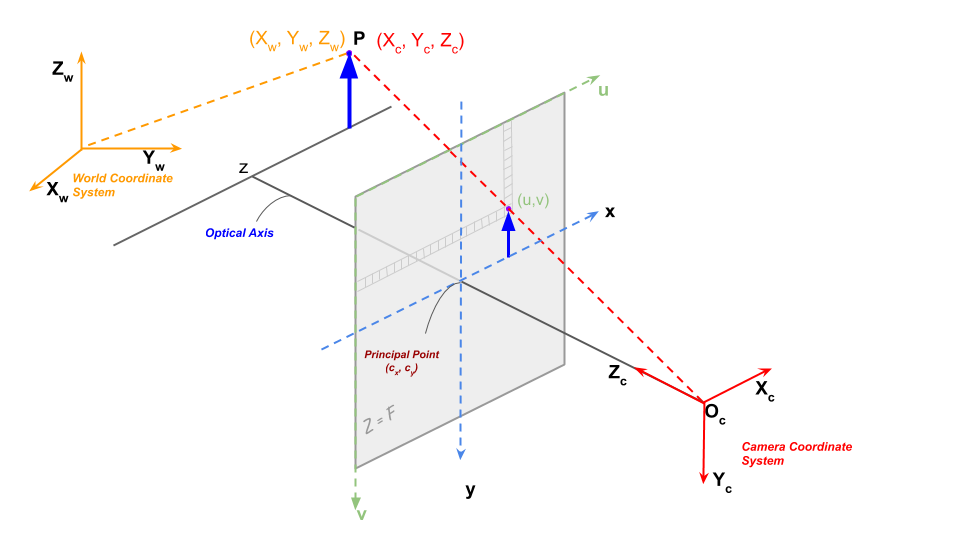
\includegraphics[width=\textwidth]{figures/projection.png}
    \caption{Projection of point \(P\) from world coordinates to camera, image and pixel coordinates, as modeled by a pinhole camera (source \cite{mallick_2020}).}
    \label{fig:projection}
\end{figure}

In our case, given the estimated distance to camera \(z_j\), image coordinates \(x_j, y_j\), depth image \(D\) dimensions \((w, h)\) and camera intrinsic parameters \(f_x, f_y, c_x, c_y\), we get the 3D camera coordinates of each joint \(j\) as:
\begin{equation}
    X_{j, cam} = \frac{(w - x_j - c_x) * z_j}{f_x}
\end{equation}\label{eq:3d_coordinates_x}
\begin{equation}
    Y_{j, cam} = \frac{(h - y_j - c_y) * z_j}{f_y}
\end{equation}\label{eq:3d_coordinates_y}
\begin{equation}
    Z_{j, cam} = z_j
\end{equation}\label{eq:3d_coordinates_z}
If extrinsic camera parameters are also provided, these camera coordinates can be projected to real-world coordinates. However, camera coordinates are enough for the performance evaluations and demos presented in this work.

\subsection{Outlier rejection}\label{subsec:outlier_rejection}
As we already mentioned in Section~\ref{subsec:minima_filter}, we might find outliers in our predicted 3D coordinates due to inconsistencies in the depth maps and noisy 2D estimations. Some of these outliers are so clear that they can be rejected with very intuitive sanity checks. It is important to note that simply rejecting these outliers would be unacceptable if no further processing was performed on the estimations. However, thanks to the \emph{Kalman} filtering presented in next section, we can replace rejected estimations for a joint with predictions yielded by its \emph{Kalman} filter based on results from previous frames.

For our application, we will consider two criteria for identifying outliers: based on the distance of the joints to the body center and based on their motion speed between consecutive frames.

\subsubsection{Based on distance to body center}
Taking as body center the estimated 3D coordinates for the pelvis center, we reject any joint with an estimated distance to that particular point higher than 150cm. This threshold has been imposed taking into account the common range of heights in adult humans (around 95\% of population height lies between 150 and 190cm~\cite{roser2013human}). We choose as reference the pelvis estimation as it is rarely occluded and, even if the estimation is a bit off, is very unusual to have strong deviations from its true location. In that way, we try to ensure a more robust outlier rejection.

\subsubsection{Based on per-joint velocity}
Another easy way to check whether a joint has been erroneously estimated or not is validating the amount of displacement between frames. We reject any joint with a displacement between frames higher than 50cm, \eg if we assume a frame rate of 20 \gls{fps}, that would be a velocity higher than 10m/s.

\subsection{\emph{Kalman} Filtering}\label{subsec:kalman_filtering}
Until this point of the process, human joints locations are estimated in a \emph{frame-by-frame} manner, without imposing any temporal dependency. In order to reduce noise and uncertainty in the 3D coordinates estimated by our method when applied to RGBD video sequences, we use an independent \emph{Kalman} filter~\cite{kalman1960new} for each joint in the skeleton.

\emph{Kalman} filters are a very powerful tool for filtering linear continuous data at a very low computational cost, both in terms of memory and time, which makes them suitable for embedded applications that must work in real-time. In a nutshell, they provide estimates of unknown or hidden variables given their uncertain measurements observed along time. Besides their lightweight implementation, another key advantage of \textit{Kalman} filters is that they do not need labeled training data of any kind to make their estimates. A great limitation of this algorithm is that for obtaining an optimal result, \textit{Gaussian} noise is assumed.

As it is shown in Figure~\ref{fig:kalman}, at each time step the algorithm performs two stages: prediction and update. During prediction, an estimate of the state of the variables defined is given depending on the physical model imposed by means of a transition matrix, the previous measurement and predictions and its uncertainty matrix. With each new measurement, both the state of the system and its uncertainty are updated and a new prediction is yielded. In our case, the state vector is formed by the three-dimensional location of each human joint estimated.

\begin{figure}[h]
    \centering
    
\includegraphics[width=\textwidth]{figures/kalman.png}
    \caption{Definition of the \emph{Kalman} filter algorithm in terms of its prediction and update stages~\cite{petteri_2011}.}
    \label{fig:kalman}
\end{figure}

In this work, we have used the \emph{pykalman} library for \emph{Python} for implementing \emph{Kalman} filters~\cite{pykalman}. It provides a very intuitive interface and allows returning predictions even if no new measurement is provided. We leverage this property for yielding new estimations for joints that have been marked as missing by our outlier rejection mechanisms. In order to avoid too much spatial drifting caused by these missing estimations, if no measurement is provided during \(n\) consecutive frames for a given joint, its \emph{Kalman} filter is reinitialized as soon as a new estimation is available. In our tests, we have set \(n\) to 4 frames.
\lhead[]{CHAPTER \thechapter. EXPERIMENTS}
\chapter{Experiments}\label{ch:experiments}
Each component of the system described in the previous chapter has its own influence in the performance of the whole method proposed in this work. We have yet to discover if their inclusion in the 3D human pose estimation pipeline is justified. Furthermore, we have to show how our lightweight algorithm compares with more complex solutions in the literature, and discuss if we have reached a fair trade-off between computational costs and accuracy.

For that purpose, we have performed both quantitative and qualitative evaluations. In this chapter, we show and discuss the results obtained for both of them. We will start presenting the publicly available dataset we have used as benchmark for both 2D and 3D pose estimations. Then, we will define the figures of merit used for evaluating 2D estimations and analyze the different results achieved by each of the methods described in Section~\ref{sec:2d_estimation}. Regarding 3D estimation, relevant figures of merit will be defined too and used to evaluate the effects of the mechanisms described in Section~\ref{sec:3d_estimation}. Quantitative evaluation will be concluded with a thorough comparison of our method against a \gls{sota} solution, both in terms of accuracy and computational costs. Last but not least, a demonstration of our system working in real-time will be presented, which will help us to validate whether our system is suitable as a component for robotics applications.

\section{Benchmark dataset}\label{sec:benchmark_dataset}
For quantiative evaluation, we will use as benchmark the publicly available \gls{bmhad}~\cite{ofli2013berkeley}. This database is comprised of synchronized data from multiple color cameras, \emph{Kinect} sensors, accelerometers, microphones and a \gls{mocap} system. From all of these, we will use \emph{Kinect} RGBD videos as input data for evaluation and \gls{mocap} data as ground-truth. The database is divided into scenes recorded from 12 subjects performing 11 different actions, with 5 repetitions per action. In other words, a total number of 660 scenes are provided. Each of these scenes has a varying length, adding up to 82 minutes of recording. As the database provides data from two \emph{Kinect} cameras capturing the scene from different viewpoints, we will include a total number of 1320 scenes in our analysis. In Figure~\ref{fig:bmhad_setup}, a diagram of the set-up used for capturing these scenes is presented.

\begin{figure}[h]
    \centering
    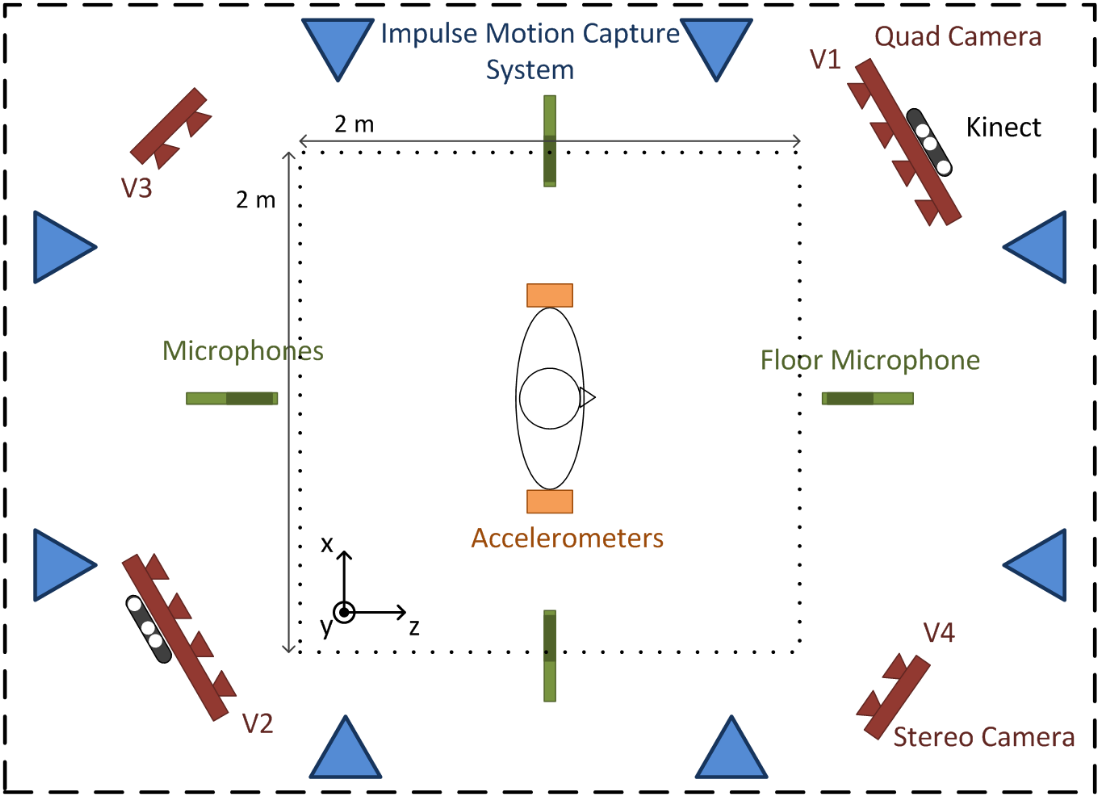
\includegraphics[width=\textwidth]{figures/bmhad_setup.png}
    \caption{Diagram of the data acquisition set-up used for building BMHAD~\cite{ofli2013berkeley}.}
    \label{fig:bmhad_setup}
\end{figure}

After studying other public datasets published in the last years, we found \gls{bmhad} to be the only one that satisfies our needs. First of all, most of the \emph{large-scale} datasets in the literature are focused on 2D pose estimation (\eg MPII~\cite{andriluka20142d} and \emph{Leeds Sports Pose}~\cite{Johnson10}). Among those containing 3D annotations, it is very hard to find registered RGB and depth images, which is a major requirement for our algorithm. That is the case of the prominent \emph{Human3.6M}~\cite{ionescu2013human3} and \emph{HumanEva}~\cite{sigal2010humaneva} datasets. Besides that, a lot of datasets with 3D information are more oriented to serve as input for action recognition tasks, and the joint locations are estimated with \glspl{sdk} provided by the manufacturers of the RGBD cameras, instead of high accuracy locations as provided by a professional \gls{mocap} system. Such is the case of the \emph{Cornell Activity Datasets}~\cite{sung2011human}. Taking all of these factors into account, the only \emph{large-scale} dataset that provides high-quality annotated joint locations registered and synchronized with both RGB and depth images is the \gls{bmhad}.

Originally, the \gls{bmhad} dataset provides labels for 21 joints extracted from the raw \gls{mocap} data. However, our final estimations depend on the 2D keypoints given by the models presented in Section~\ref{sec:2d_estimation}, which have been trained with samples from the MPII dataset. In order to make our results comparable with \gls{bmhad} labels, we have reduced the number of joints provided to 12: head, shoulders, elbows, hands, pelvis, knees and feet. For head and pelvis, some modifications to the original labels have been performed in order to match \gls{bmhad} and MPII definitions. In the case of the head label, the \textit{HeadEnd} and \textit{Head} labels in \gls{bmhad}, and the \textit{head top} and \textit{upper neck} labels in MPII  have been averaged, respectively, in order to get a unique comparable head keypoint. In the case of the pelvis label, the \textit{LeftUpLeg} and \textit{RightUpLeg} labels in \gls{bmhad} and the \textit{l hip} and \textit{r hip} labels in MPII have been averaged as well. For the latter, merging left and right hips labels has been necessary because of slightly different definitions in terms of what is considered \textit{hip} or \textit{UpLeg} in each of the datasets, looking much more similar between them after the averaging process. In Figure~\ref{fig:bmhad_labels}, a visual comparison between the original \gls{bmhad} labels and the result of our transformation is shown.

\begin{figure}[h]\centering
    \begin{subfigure}{0.47\textwidth}\centering
        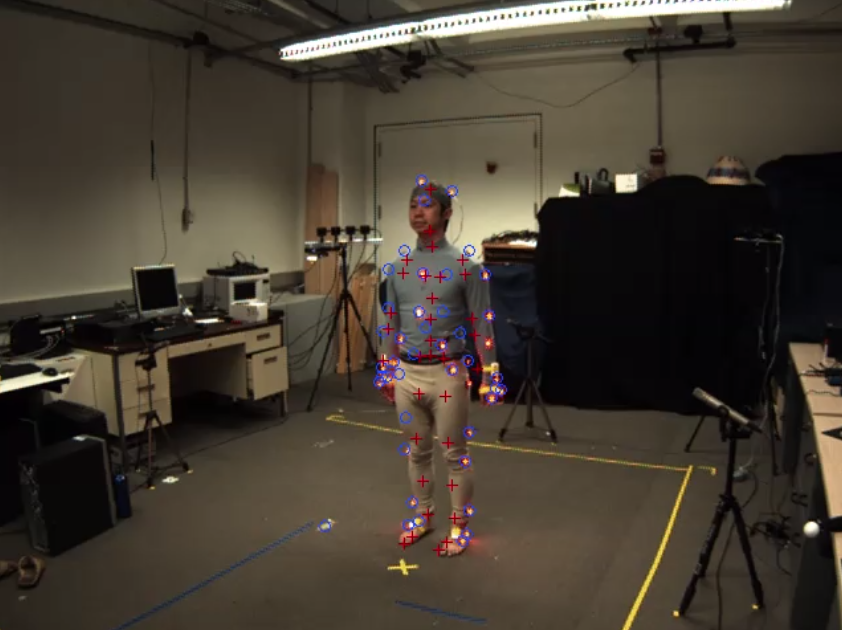
\includegraphics[height=5.75cm]{figures/labels_original.png} 
        \caption{Original BMHAD labels (red crosses).}
        \label{subfig:cp_general}
    \end{subfigure}
    \begin{subfigure}{0.51\textwidth}\centering
        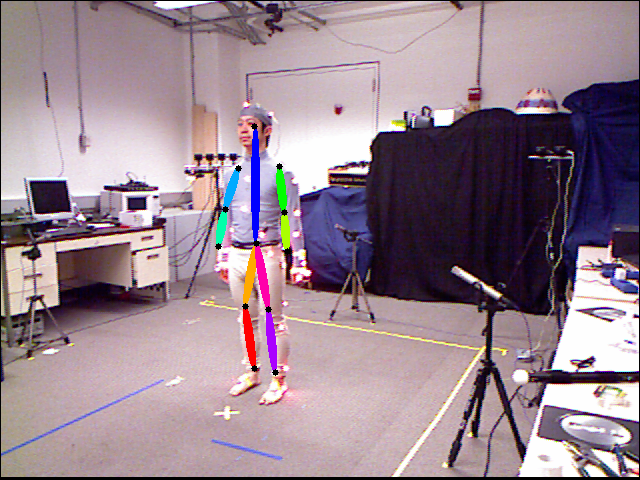
\includegraphics[height=5.75cm]{figures/labels_modified.png}
        \caption{Modified labels with joints linked.}
        \label{subfig:cp_particular}
    \end{subfigure}
    \caption{In order to compare our results with the labels provided by BMHAD, we have transformed the original keypoints shown in (a) to the simpler configuration shown in (b). Please note that in (a) markers used for MoCap and final keypoints are shown in blue and red, respectively. Also, (a) and (b) show the same moment in time, but captured with different cameras.}
    \label{fig:bmhad_labels}
\end{figure}

It is worth mentioning that a major limitation of using \gls{bmhad} for assessing our performance is its lack of scenes \emph{in the wild}. This is an issue with no easy solution for the field of 3D human pose estimation, as precise labels can only be captured by means of cumbersome \gls{mocap} systems, which can hardly be used in more natural scenarios. Besides that, the dataset only provides two different points of view, so further research in terms of how our system performs under more intricate perspectives can only be done qualitatively. Another issue we have discovered is that, for frames with fast motions, \gls{mocap} labels might be displaced, as it can be seen in the left hand of the subject in Figure~\ref{fig:wrong_hands}. Even though this effect might slightly drop our accuracy, it will equally affect every method tested and so comparisons will still be well-founded.

\begin{figure}[h]\centering
    \begin{subfigure}{0.49\textwidth}\centering
        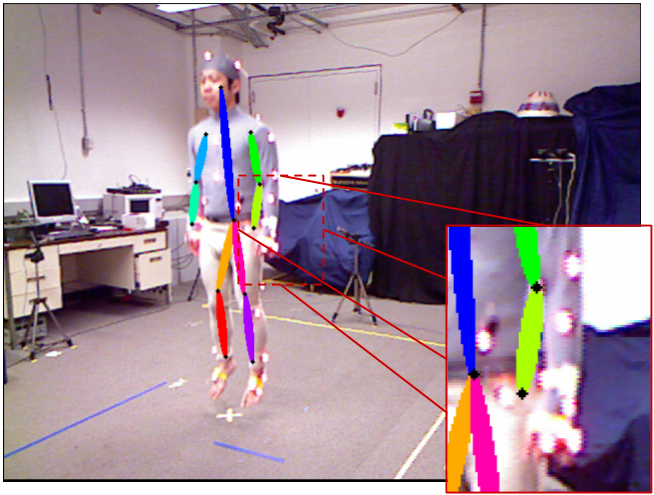
\includegraphics[height=5.75cm]{figures/2d_gt.png} 
        \caption{Original BMHAD label projected in 2D.}
        \label{subfig:2d_gt}
    \end{subfigure}
    \begin{subfigure}{0.49\textwidth}\centering
        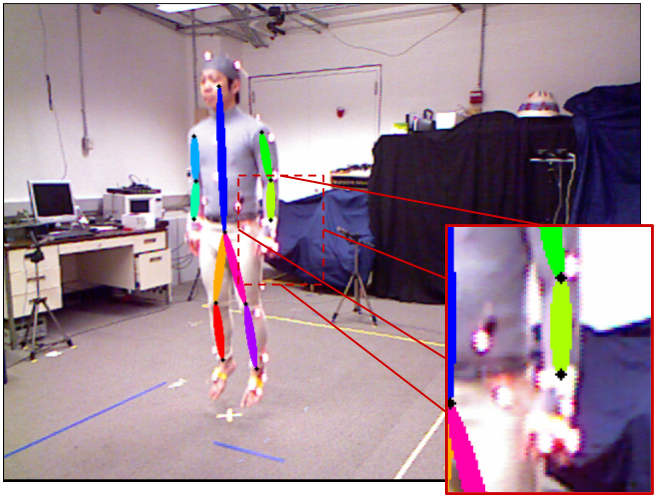
\includegraphics[height=5.75cm]{figures/2d_cpm.png}
        \caption{Joints estimated using CPMs.}
        \label{subfig:2d_cpm}
    \end{subfigure}
    \caption{In scenes with rapid movements, such as \textit{a01}, BMHAD labels might suffer some displacements. In (a), this effect is demonstrated to be significant for the left hand label. In (b), the corresponding estimation is shown.}
    \label{fig:wrong_hands}
\end{figure}

In order to provide a more intuitive interpretation of the results, the different actions considered in the dataset have been classified in terms of their dynamics and the occlusion degree of the human body joints, as follows:

\begin{itemize}
    \item \textbf{High dynamics and heavily occluded}: Bending (\textit{a03}) and throwing ball (\textit{a08}). From now on, results for these actions will be presented in \textit{red}.
    \item \textbf{High dynamics and slightly occluded}: Jumping in place (\textit{a01}), jumping jacks (\textit{a02}) and boxing (\textit{a04}). From now on, results for these actions will be presented in \textit{orange}.
    \item \textbf{Low dynamics and heavily occluded}: Sit down then stand up (\textit{a09}), sit down (\textit{a10}) and stand up (\textit{a11}). From now on, results for these actions will be presented in \textit{green}.
    \item \textbf{Low dynamics and slightly occluded}: Waving with two hands (\textit{a05}), waving with one hand (\textit{a06}) and clapping hands (\textit{a07}). From now on, results for these actions will be presented in \textit{blue}.
\end{itemize}

\section{2D Estimation quantitative evaluation}\label{sec:2d_estimation_evaluation}
Following the approach of many works in the literature, the person detection and subsequent pose estimation tasks are decoupled. For evaluation purposes, we will assume that a bounding box fitted around the subject can be inferred from the ground-truth. More precisely, we compute the center of the human pose as the average location between all the joints and crop a squared region around it, which is 1.25 times bigger than the biggest difference between joints in \(x\) or \(y\) dimensions. It is important to note that these bounding boxes have been resized for each method evaluated according to the sizes defined in their respective articles: 368 pixels for \glspl{cpm} and 256 pixels for both \gls{sh} and \glspl{cp}.

As mentioned in Section~\ref{sec:benchmark_dataset}, we will use \gls{bmhad} for evaluation. However, as \gls{bmhad} only provides labels in 3D coordinates, we have projected the 3D joint locations into the RGB video sequences using the camera calibration parameters included in the dataset. For this evaluation, both our estimations and the ground-truth labels have been converted to the 12 joints model described in the previous section.

\subsection{Figures of merit}\label{subsec:2d_metrics}
The performance of the 2D pose estimation approaches presented in Section~\ref{sec:2d_estimation} has been evaluated according to the \gls{pckh} indicator~\cite{andriluka20142d}. According to the \gls{pckh} score, the estimation of the joint position is considered to be correct if the distance between the estimated and the ground-truth joint locations is below a threshold dependant on the head segment length. The threshold is usually indicated after the \textit{at} symbol, thus for a \gls{pckh}@0.1, we would consider as correct keypoints those with an error lower than the 10\% of the head link size.

For the results presented in this report, the head segment length is obtained for each frame from the corresponding ground-truth. The \gls{pckh} score is computed for each joint considering all the frames in the same video sequence for thresholds ranging between 0 and 1 head segment lengths. Regarding missing joints, they are considered to be wrong regardless of the threshold. 

\subsection{Experimental results}\label{subsec:2d_experimental_results}
For the 2D estimation evaluation, results per joint and action are presented for the three methods tested: \glspl{cpm}~\cite{Wei2016-rb}, \gls{sh}~\cite{Newell2016-cy} and \gls{cp}~\cite{Gkioxari2016-ix}. As it can be seen in Figure~\ref{fig:pckh_2d}, these methods show similar performance with respect to each other regardless of the human joint. Having said that, \glspl{cpm} perform slightly better than the other two for every joint if we set the threshold to the length of one head segment (\gls{pckh}@1), with a mean score of 95.85\% of parts correctly detected (see Table~\ref{tab:pckh_2d}). Regarding the differences in performance between joints, hand locations are harder to disambiguate than any other joint, with a mean \gls{pckh}@1 below 90\% in every method tested. This can be justified by the higher level of occlusion they might have in comparison with other joints. Besides that, hands are the joints with higher dynamics in the actions included in the dataset, and labels might be displaced as we previously mentioned in Section~\ref{sec:benchmark_dataset}. Figure~\ref{fig:wrong_hands} presents an example of a misplaced hand label, along with our estimation.

\begin{figure}[h]
    \centering
    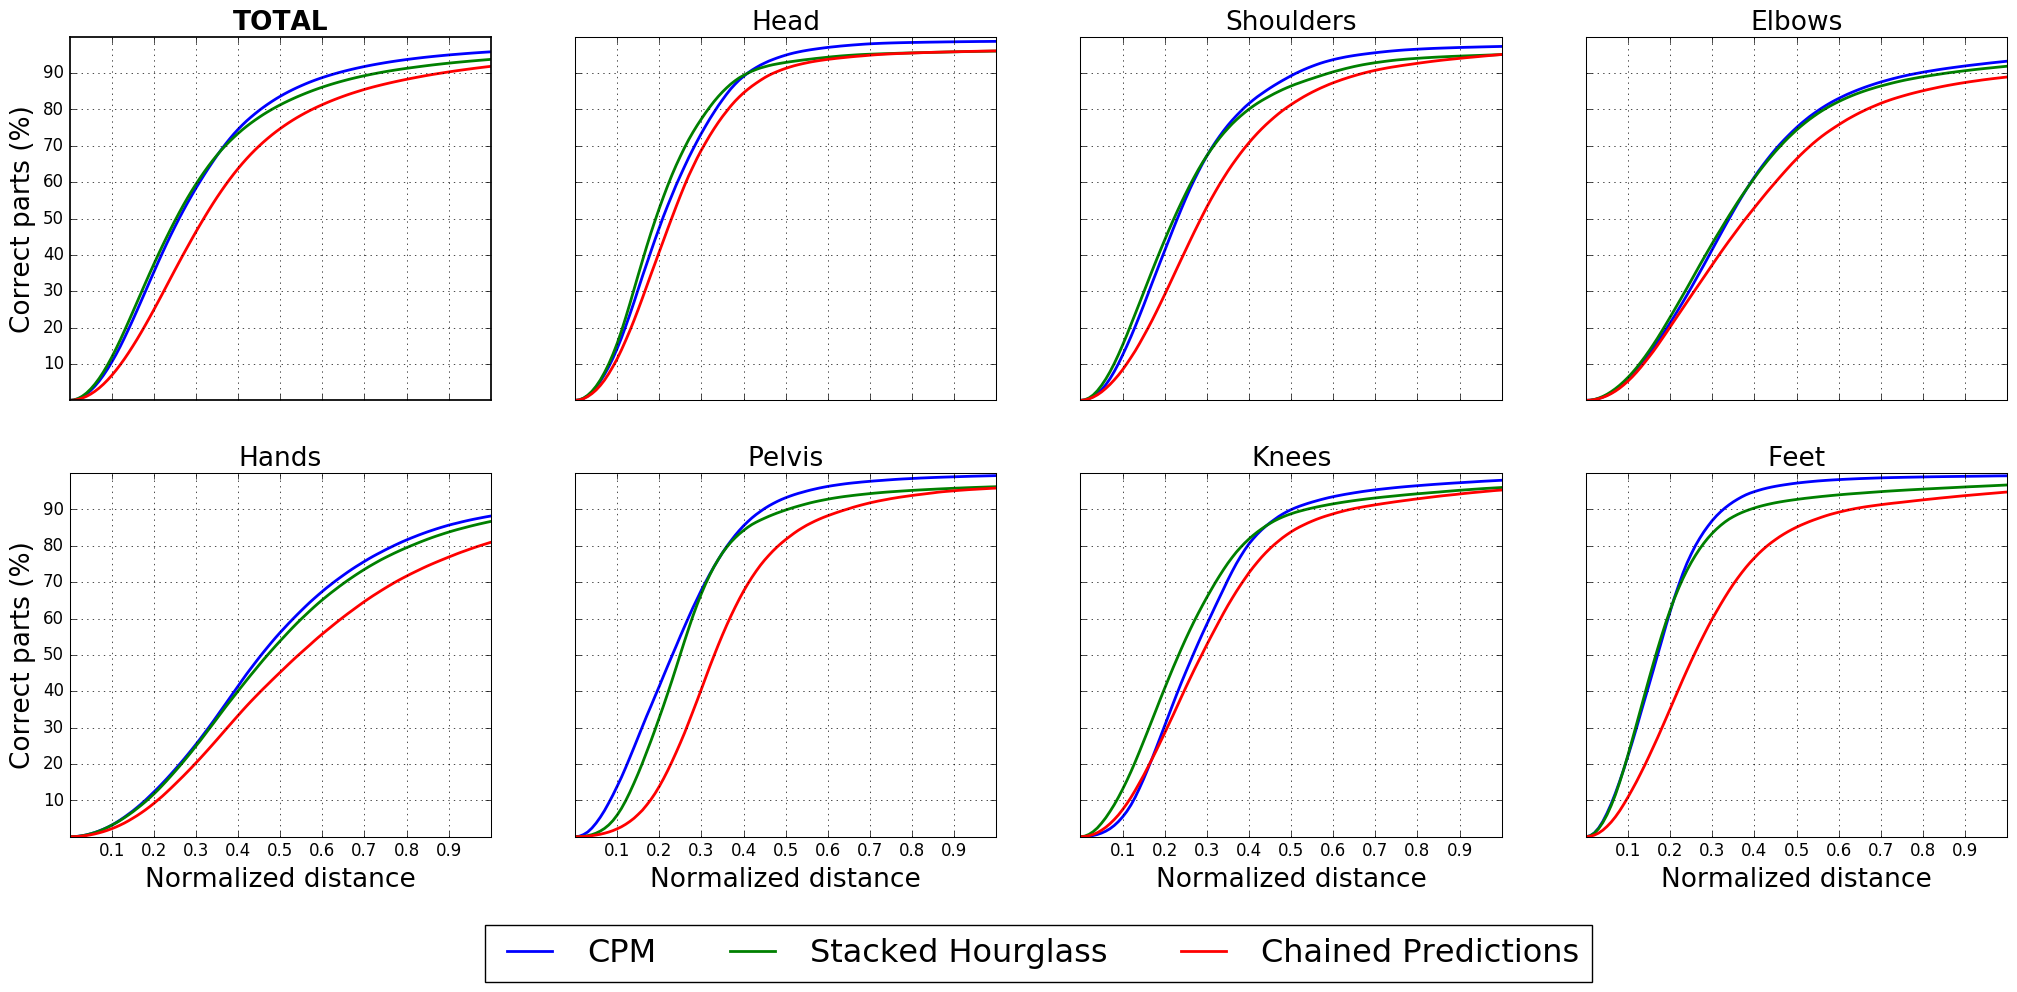
\includegraphics[width=\textwidth]{figures/pckh_2d.png}
    \caption{Quantitative 2D pose estimation results on BMHAD per joint, using as figure of merit PCKh 2D~@~0-1~(\%). }
    \label{fig:pckh_2d}
\end{figure}

\begin{table}[!ht]  
  \centering
  \resizebox{\textwidth}{!}{\begin{tabular}{l||ccccccc|c}
    \hline
    & Head & Shoulders & Elbows & Hands & Pelvis & Knees & Feet & TOTAL \\
    \hline
    \glspl{cpm} & \textbf{98.73} & \textbf{97.34} & \textbf{93.28} & \textbf{88.20} & \textbf{99.31} & \textbf{98.03} & \textbf{99.26} & \textbf{95.85} \\
    \gls{sh} & 96.06 & 95.11 & 91.89 & 86.71 & 96.26 & 96.04 & 96.74 & 93.77 \\
    \glspl{cp} & 96.11 & 95.12 & 88.93 & 80.97 & 95.88 & 95.35 & 94.80 & 91.86 \\
    \hline
  \end{tabular}}
  \caption{Quantitative 2D pose estimation results on BMHAD per joint, using as figure of merit PCKh~2D~@~1~(\%). Values in bold correspond to the best results achieved for each category.}
  \label{tab:pckh_2d}
\end{table}

\begin{table}[!ht]  
  \centering
  \resizebox{\textwidth}{!}{\begin{tabular}{l||oorobbbrggg|c}
    \hline
    & a01 & a02 & a03 & a04 & a05 & a06 & a07 & a08 & a09 & a10 & a11 & TOTAL \\
    \hline
    \glspl{cpm} & 97.98 & 96.90 & \textbf{87.49} & \textbf{97.04} & \textbf{98.23} & \textbf{97.26} & \textbf{99.30} & \textbf{96.25} & \textbf{98.04} & \textbf{97.14} & \textbf{98.16} & \textbf{95.85} \\
    \gls{sh} & \textbf{98.35} & \textbf{98.40} & 80.42 & 96.30 & 97.42 & 95.80 & 97.91 & 93.96 & 96.77 & 94.73 & 96.13 & 93.77 \\
    \glspl{cp} & 96.55 & 94.07 & 77.69 & 95.06 & 94.05 & 93.71 & 97.40 & 93.34 & 96.19 & 92.60 & 95.64 & 91.86 \\
    \hline
  \end{tabular}}
  \caption{Quantitative 2D pose estimation results on BMHAD per action, using as figure of merit PCKh~2D~@~1~(\%). Values in bold correspond to the best results achieved for each category. Columns are colored following the convention established in Section~\ref{sec:benchmark_dataset}.}
  \label{tab:pckh_2d_action}
\end{table}

\begin{table}[!ht]  
  \centering
  \resizebox{\textwidth}{!}{\begin{tabular}{l||ro|gb}
    \hline
    & \multicolumn{2}{c|}{High Dynamics} & \multicolumn{2}{c}{Low Dynamics} \\
    \cline{2-5}
    & Heavily Occluded & Slightly Occluded & Heavily Occluded & Slightly Occluded \\
    \hline
    \glspl{cpm} & \textbf{91.87} & 97.31 & \textbf{97.78} & \textbf{98.26} \\
    \gls{sh} & 87.19 & \textbf{97.68} & 95.88 & 97.04 \\
    \glspl{cp} & 85.52 & 95.22 & 94.81 & 95.05 \\
    \hline
  \end{tabular}}
  \caption{Quantitative 2D pose estimation results on BMHAD per action type,  using as figure of merit PCKh~2D~@~1~(\%). Values in bold correspond to the best results achieved for each category. Columns are colored following the convention established in Section~\ref{sec:benchmark_dataset}.}
  \label{tab:pckh_2d_action_type}
\end{table}

The relation between the actions performed in the evaluated scenes and the results in the 2D pose estimation for each method are presented in both Table~\ref{tab:pckh_2d_action} and Table~\ref{tab:pckh_2d_action_type}. In the latter, the actions have been grouped in terms of dynamics and occlusion, as described in Section~\ref{sec:benchmark_dataset}. Taking a look at Table~\ref{tab:pckh_2d_action}, it can be concluded that, in general, \glspl{cpm} performs better than SH and CPs, as it gets a significantly better score for most of the actions. Besides, as presented in Table~\ref{tab:pckh_2d_action_type}, all methods perform similarly for actions with low dynamics and/or slightly occluded joints, with a difference of only $\pm3\%$ in the final score. However, there is a much greater gap in performance when the scenes with the hardest actions are evaluated, \ie heavily occluded actions with high dynamics. For this kind of actions, \glspl{cpm} get a \gls{pckh}@1 of 91.87\%, while SH and CPs achieve a 87.19\% and 85.52\% of correct parts, respectively. This is a very relevant result . As \gls{bmhad} has been captured in a controlled environment, determining which method performs better under adverse circumstances can give us an idea of how these methods would perform in the real world. Figure~\ref{fig:2d_comparison} displays an example where \glspl{cpm} outperforms its competitors when estimating a very challenging pose.

\begin{figure}[h]\centering
    \begin{subfigure}{0.32\textwidth}\centering
        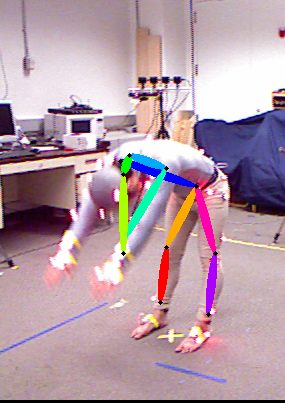
\includegraphics[height=7.cm]{figures/chained_failed.png} 
        \caption{CPs failed estimation.}
        \label{subfig:chained_failed}
    \end{subfigure}
    \begin{subfigure}{0.32\textwidth}\centering
        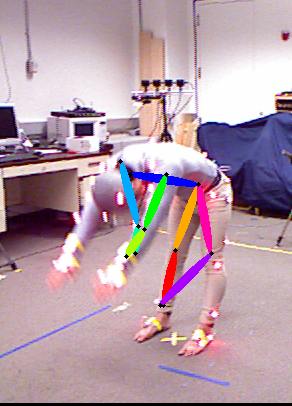
\includegraphics[height=7.cm]{figures/stacked_failed.png}
        \caption{SH failed estimation.}
        \label{subfig:stacked_failed}
    \end{subfigure}
    \begin{subfigure}{0.32\textwidth}\centering
        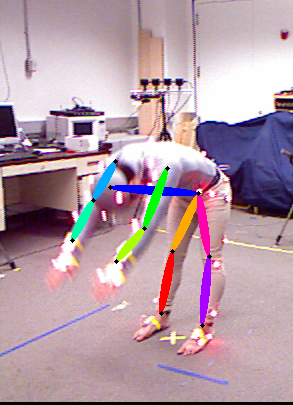
\includegraphics[height=7.cm]{figures/cpm_right.png}
        \caption{CPMs accurate estimation.}
        \label{subfig:cpm_right}
    \end{subfigure}
    \caption{In challenging scenes like \textit{a03}, with high dynamics and occlusions, CPMs (c) outperform CPs (a) and SH (b) methods. }
    \label{fig:2d_comparison}
\end{figure}

\section{3D Estimation quantitative evaluation}\label{sec:3d_estimation_evaluation}
For 3D estimation, we will rely again on the labels provided by the \gls{mocap} data included in the \gls{bmhad} dataset. For simplicity, all of the estimations generated in this work are given in camera coordinates. Taking that into account, the corresponding \gls{bmhad} labels have been transformed from world to camera coordinates for the evaluation. Also, following the same strategy described in the previous section, both estimations and ground-truth labels have been further transformed to match our 12 joints model defined in Section~\ref{sec:benchmark_dataset}. It is important to note that these transformations have been applied on the final 3D estimations, but the 2D estimations used as input have preserved their original MPII joints definition. In that way, we can fairly compare our results with those provided by other methods that might have been trained for 3D estimation with different label definitions.

\subsection{Figures of merit}
The performance of the 3D estimation methods presented in this work has been evaluated using the \gls{mpjpe} and the 3D version of the \gls{pckh} score, already described in Section~\ref{subsec:2d_metrics}. \gls{mpjpe} is simply defined as the average \emph{Euclidean} distance between the prediction for the joints location  in the skeleton and their respective ground-truths. Regarding the \gls{pckh} score, we use the same definition presented in the previous section, being the only difference that the head link segment length will be extracted from the three-dimensional data in terms of real-world distance, instead of pixels in a 2D image. 

\subsection{Experimental results}
In order to assess the effectiveness of our method for 3D estimation described in Section~\ref{sec:3d_estimation}, we compare the \gls{mpjpe} obtained using as baseline the direct 3D estimation from the 2D keypoints, without any filtering. For this test, we have used \glspl{cpm} as 2D estimator, since it is the most accurate among the evaluated ones, as we demonstrated in Section~\ref{subsec:2d_experimental_results}. We have selected a subset of 132 scenes from the \gls{bmhad} dataset, containing every action performed by every subject, but only its first repetition and captured with the first of the \emph{Kinect} sensors.

As it can be shown in Table~\ref{tab:mpjpe_joint_baseline}, the overall performance of the 3D pose estimation improves significantly with the inclusion of the processing steps described in Section~\ref{sec:3d_estimation}. Specifically, the total \gls{mpjpe} gets reduced in half. It is important to note that this difference is mostly driven by the results obtained for the joints that belong to the upper body. For most of the actions in the dataset, these joints are the ones with higher dynamics and self-occlusions, which brings to light how our algorithm is able to perform under these circumstances when compared with a direct inference. When \textit{pelvis}, \textit{knees} and \textit{feet} get compared, the baseline results are slightly better. As these joints are less challenging to estimate throughout the scenes in the dataset, our mechanisms can actually distort their locations to some extent. For instance, if both the depth map and the 2D estimation are completely accurate, our minima filter could pick a location which is closer to the camera that it actually is. Nonetheless, this mechanism is very effective for correcting errors when the conditions are not ideal.

\begin{table}[!ht]  
  \centering
  \resizebox{\textwidth}{!}{\begin{tabular}{l||ccccccc|c}
    \hline
    & Head & Shoulders & Elbows & Hands & Pelvis & Knees & Feet & TOTAL \\
    \hline
    Baseline & 1413.2 & 194.5 & 164.0 & 355.5 & \textbf{174.9} & \textbf{90.5} & \textbf{65.8} & 277.4 \\
    Ours & \textbf{104.2} & \textbf{146.3} & \textbf{125.6} & \textbf{137.6} & 198.2 & 103.7 & 79.0 & \textbf{123.9} \\
    \hline
  \end{tabular}}
  \caption{Quantitative 3D pose estimation results on BMHAD per joint, compared against our baseline, using as figure of merit MPJPE (mm). Values in bold correspond to the best results achieved for each category.}
  \label{tab:mpjpe_joint_baseline}
\end{table}

In that sense, it is worth discussing in detail the great difference for the \textit{head} joint. In that particular case, as we explained in Section~\ref{sec:benchmark_dataset}, the labels get transformed after 3D estimation, but the original 2D estimations are yielded in MPII format, which gives two different labels for the head of the subject: \textit{upper neck} and \textit{head top}. The latter is placed right above the head, which makes the 3D estimation consistently fail if no further processing is applied. Thanks to our minima filter, this error gets dramatically reduced. An example of such case can be seen in Figure~\ref{fig:head}.

\begin{figure}[h]
    \centering
    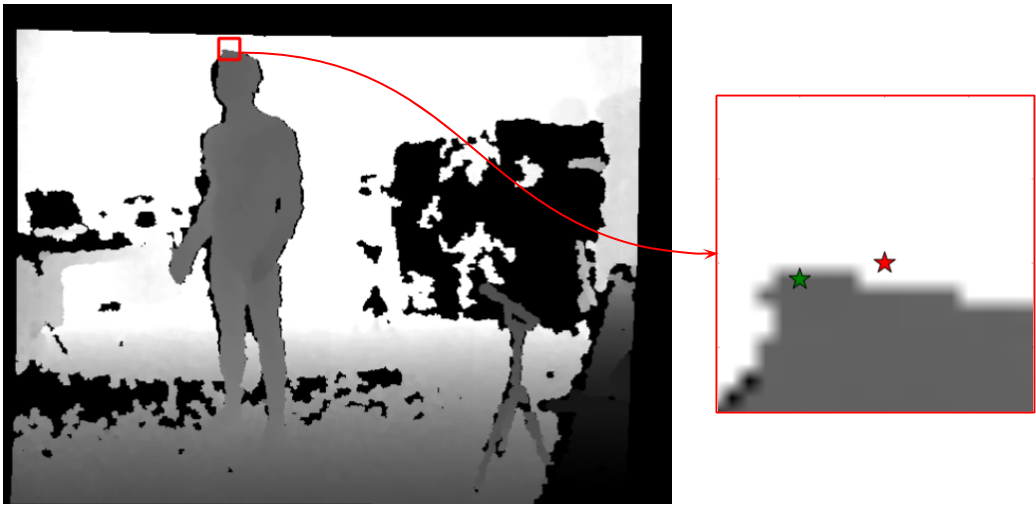
\includegraphics[width=\textwidth]{figures/head.png}
    \caption{Small deviations in the 2D estimation can lead to huge differences in depth. At the left side of the figure, the depth image with the region of interest around the \textit{head top} joint. At the right side, we can see highlighted in red the original 2D estimation and in green the point we used for depth estimation after minima filter correction.}
    \label{fig:head}
\end{figure}

In order to better understand the nature of the error we get in the estimation, we have analyzed how it affects each dimension (\(X\), \(Y\), \(Z\)) independently. For this purpose, we have plotted the module of the error per joint and dimension for our 3D estimation, using once again \glspl{cpm} as 2D estimator. As we can see in Figure~\ref{fig:mpjpe_by_dim}, most of the error in the evaluation comes from the \(Z\) dimension, \ie from the estimated depth or distance to the camera. As demonstrated in Section~\ref{subsec:2d_experimental_results}, the 2D estimators tested perform very accurately, with \gls{pckh} scores up to 95\%. However, very slight deviations in the 2D estimation and self-occlusions can make huge differences in the estimated depth.

\begin{figure}[h]
    \centering
    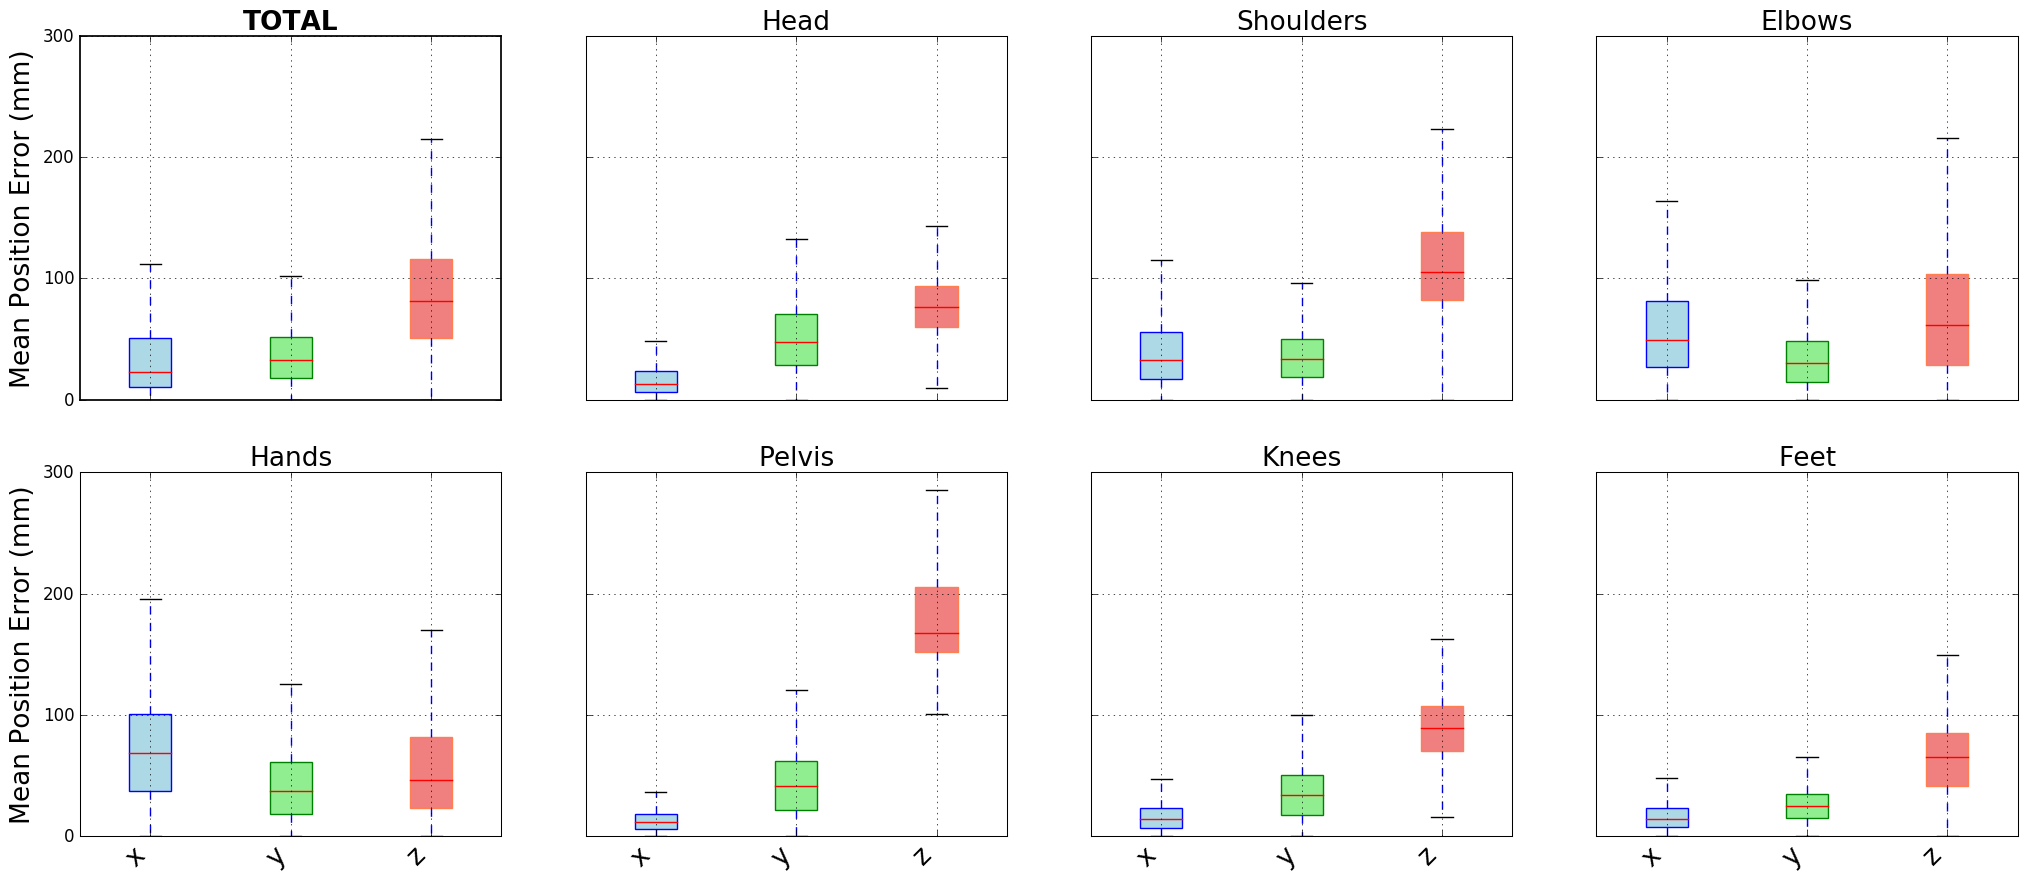
\includegraphics[width=\textwidth]{figures/mpjpe-xyz-ours.png}
    \caption{Quantitative 3D pose estimation results on BMHAD per joint, using as figure of merit the module of the difference between estimations and ground-truth for each dimension (mm).}
    \label{fig:mpjpe_by_dim}
\end{figure}

\subsection{Comparison with other methods}
Our approach follows the strategy proposed by Zimmermann \etal\cite{Zimmermann2018-sn}, in the sense that our estimations also rely on registered RGB and depth images. For detecting the 2D keypoints in the RGB images, they use a model provided by the \emph{OpenPose} library~\cite{cao2018openpose} with fixed weights. Then, an occupancy voxel grid with a resolution of about 3 cm is computed by transforming the depth map into a point-cloud and, using the calibration matrix, the initial 3D coordinates of the keypoints are estimated. The voxel grid and the 2D likelihood maps are processed by a 3D CNN which optimizes the \emph{Sum of Squared Errors} between the ground-truth and the estimated location in 3D. An overview of the architecture proposed by Zimmermann \etal can be seen in Figure~\ref{fig:zimmermann}.

\begin{figure}[h]
    \centering
    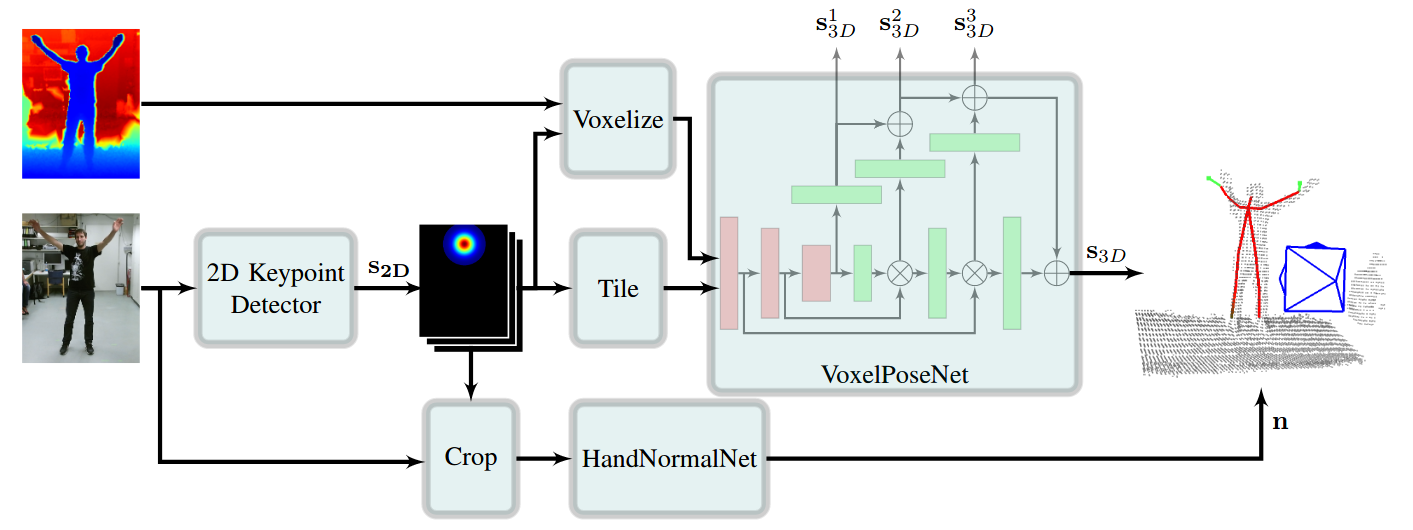
\includegraphics[width=\textwidth]{figures/zimmermann.png}
    \caption{Overview of the solution introduced by Zimmmermann \etal for 3D human pose estimation~\cite{Zimmermann2018-sn}.}
    \label{fig:zimmermann}
\end{figure}

Zimmermann \etal provided results on their own datasets, defining the skeleton as a set of 18 joints, which are based on the definition of the COCO dataset keypoints~\cite{lin2014microsoft}. In order to compare our results with those yielded by Zimmermann's approach, we have averaged their \textit{LEar} and \textit{REar} keypoints and \textit{RHip} and \textit{LHip} keypoints to get unique head and pelvis labels, respectively. By doing so, we match the modifications presented in Section~\ref{sec:benchmark_dataset} for \gls{bmhad} and MPII datasets.

For some frames in the evaluated scenes, specially in scenarios with high occlusions, Zimmermann's method did not return any estimated location for certain joints. When computing the \gls{pckh} score, as it is simply a percentage of parts correctly detected, these joints can be included in the evaluation and are taken into account as \textit{not correct}. However, as \gls{mpjpe} is defined as an average of distances, such empty estimations are invalid and must be discarded. In order to avoid a biased comparison, such joint estimations have been removed for every method when measuring the \gls{mpjpe}. For this comparison, we have used the \gls{bmhad} dataset in its entirety.

Taking a look at the \gls{pckh} curves shown in Figure~\ref{fig:pckh_3d}, we conclude that, except for the pelvis joint, the overall performance of Zimmermann's method is similar to ours, specially when using \glspl{cpm} as our 2D pose estimator. In fact, Zimmermann's method only performs better for shoulders and pelvis joints, with a total \gls{pckh}@1 of 81.55\%, versus an 80.23\% of our method with \glspl{cpm} (see Table~\ref{tab:pckh_3d_joint}). It is also important to note that, when evaluating 3D estimations with \gls{pckh}, final scores are lower than when evaluating 2D locations, as the added dimension increases the magnitude of the error, even though the head segment length also increases.

\begin{figure}[h]
    \centering
    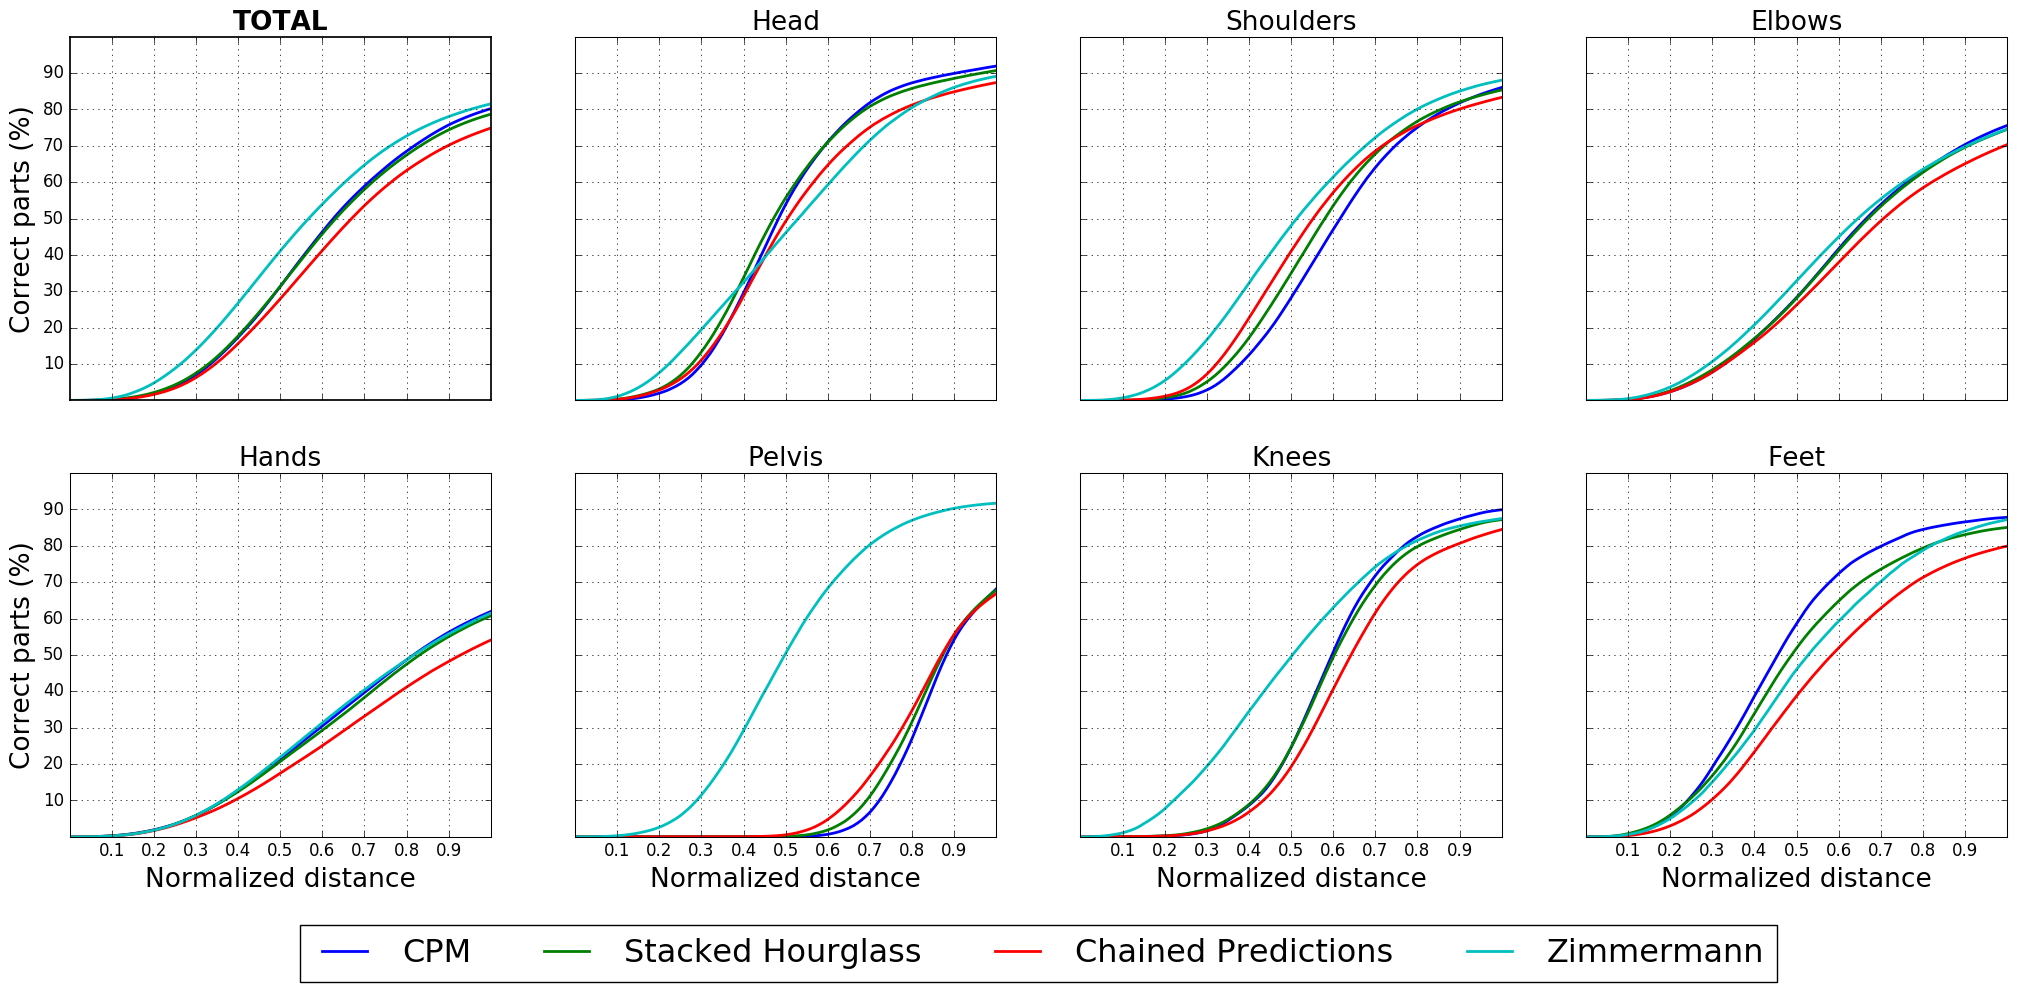
\includegraphics[width=\textwidth]{figures/pckh_3d.png}
    \caption{Quantitative 3D pose estimation results on BMHAD per joint, using as figure of merit PCKh~3D~@~0-1~(\%).}
    \label{fig:pckh_3d}
\end{figure}

\begin{table}[!ht]  
  \centering
  \resizebox{\textwidth}{!}{\begin{tabular}{l||ccccccc|c}
    \hline
    & Head & Shoulders & Elbows & Hands & Pelvis & Knees & Feet & TOTAL \\
    \hline
    \glspl{cpm} & \textbf{91.93} & 86.05 & \textbf{75.59} & \textbf{61.95} & 68.17 & \textbf{89.93} & \textbf{87.84} & 80.23 \\
    \gls{sh} & 90.71 & 85.36 & 74.54 & 60.76 & 67.85 & 87.20 & 85.06 & 78.70 \\
    \glspl{cp} & 87.41 & 83.32 & 70.33 & 54.08 & 66.87 & 84.49 & 79.94 & 74.88 \\
    Zimm. & 89.13 & \textbf{88.05} & 74.61 & 61.50 & \textbf{91.71} & 87.50 & 87.21 & \textbf{81.55} \\
    \hline
  \end{tabular}}
  \caption{Quantitative 3D pose estimation results on BMHAD per joint, using as figure of merit PCKh~3D~@~1~(\%). Values in bold correspond to the best results achieved for each category.}
  \label{tab:pckh_3d_joint}
\end{table}

If we take a look at the results obtained for the same estimations when evaluated in terms of \gls{mpjpe}, we see that the gap between our method and Zimmerman's increases. First of all, boxplots in Figure~\ref{fig:mpjpe} show that Zimmermann's method error present a lower standard deviation for most of the joints. Moreover, according to Table~\ref{tab:mpjpe_joint}, Zimmermann's mean error is lower for every joint, with the exceptions of head and feet, with a total \gls{mpjpe} of 128.1 mm, versus a \gls{mpjpe} of 144.1 mm for our method with \glspl{cpm}. 

\begin{figure}[h]
    \centering
    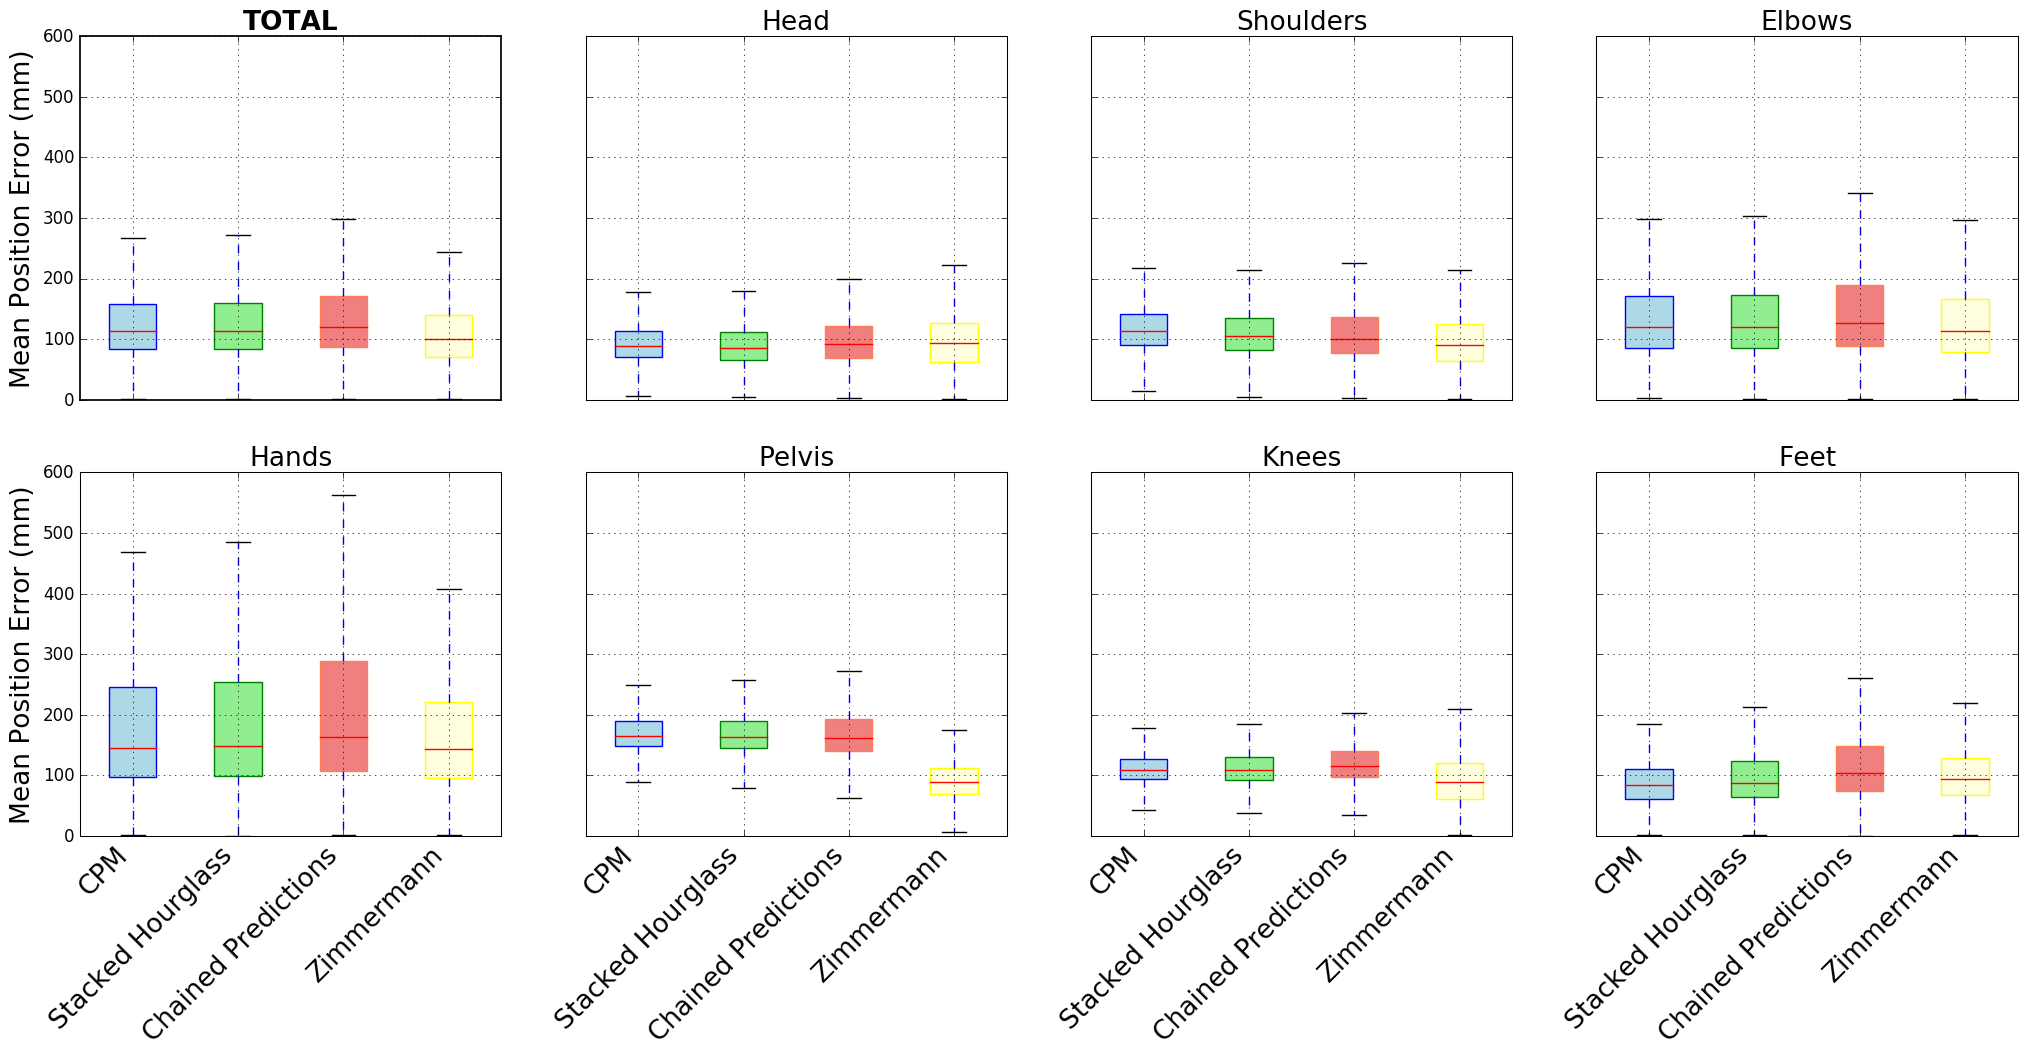
\includegraphics[width=\textwidth]{figures/mpjpe.png}
    \caption{Quantitative 3D pose estimation results on BMHAD per joint, using as figure of merit the \emph{Euclidean} distance between estimations and groun-truth (mm).}
    \label{fig:mpjpe}
\end{figure}

\begin{table}[!ht]  
  \centering
  \resizebox{\textwidth}{!}{\begin{tabular}{l||ccccccc|c}
    \hline
    & Head & Shoulders & Elbows & Hands & Pelvis & Knees & Feet & TOTAL \\
    \hline
    \glspl{cpm} & \textbf{99.5} & 129.4 & 149.9 & 200.5 & 179.9 & 132.8 & \textbf{112.5} & 144.1 \\
    \gls{sh} & 102.3 & 124.8 & 152.0 & 208.7 & 179.0 & 138.6 & 127.2 & 148.7 \\
    \glspl{cp} & 153.6 & 127.2 & 167.9 & 232.2 & 178.9 & 148.5 & 147.1 & 164.8 \\
    Zimm. & 101.2 & \textbf{102.1} & \textbf{143.5} & \textbf{198.7} & \textbf{95.1} & \textbf{108.2} & 117.7 & \textbf{128.1} \\
    \hline
  \end{tabular}}
  \caption{Quantitative 3D pose estimation results on BMHAD per joint, using as figure of merit MPJPE (mm). Values in bold correspond to the best results achieved for each category.}
  \label{tab:mpjpe_joint}
\end{table}

It is still a very competitive result for our approach, particularly taking into account its simplicity and low computational burden, which will be explored in Section~\ref{sec:computational_burden}. Also, our explicit outlier rejection and Kalman filtering plays a vital role in the final results, as evidenced by the differences shown in the \gls{pckh} and \gls{mpjpe} scores. Even when our average error in terms of distance was higher than the one yielded by Zimmermann's method, we manage to get very similar or even better percentages of correct parts, which means that joints estimated with broad error were properly identified and corrected. In Figure~\ref{fig:zimmermann_failed}, some examples of such cases are presented.

\begin{figure}[h]\centering
    \begin{subfigure}{0.49\textwidth}\centering
        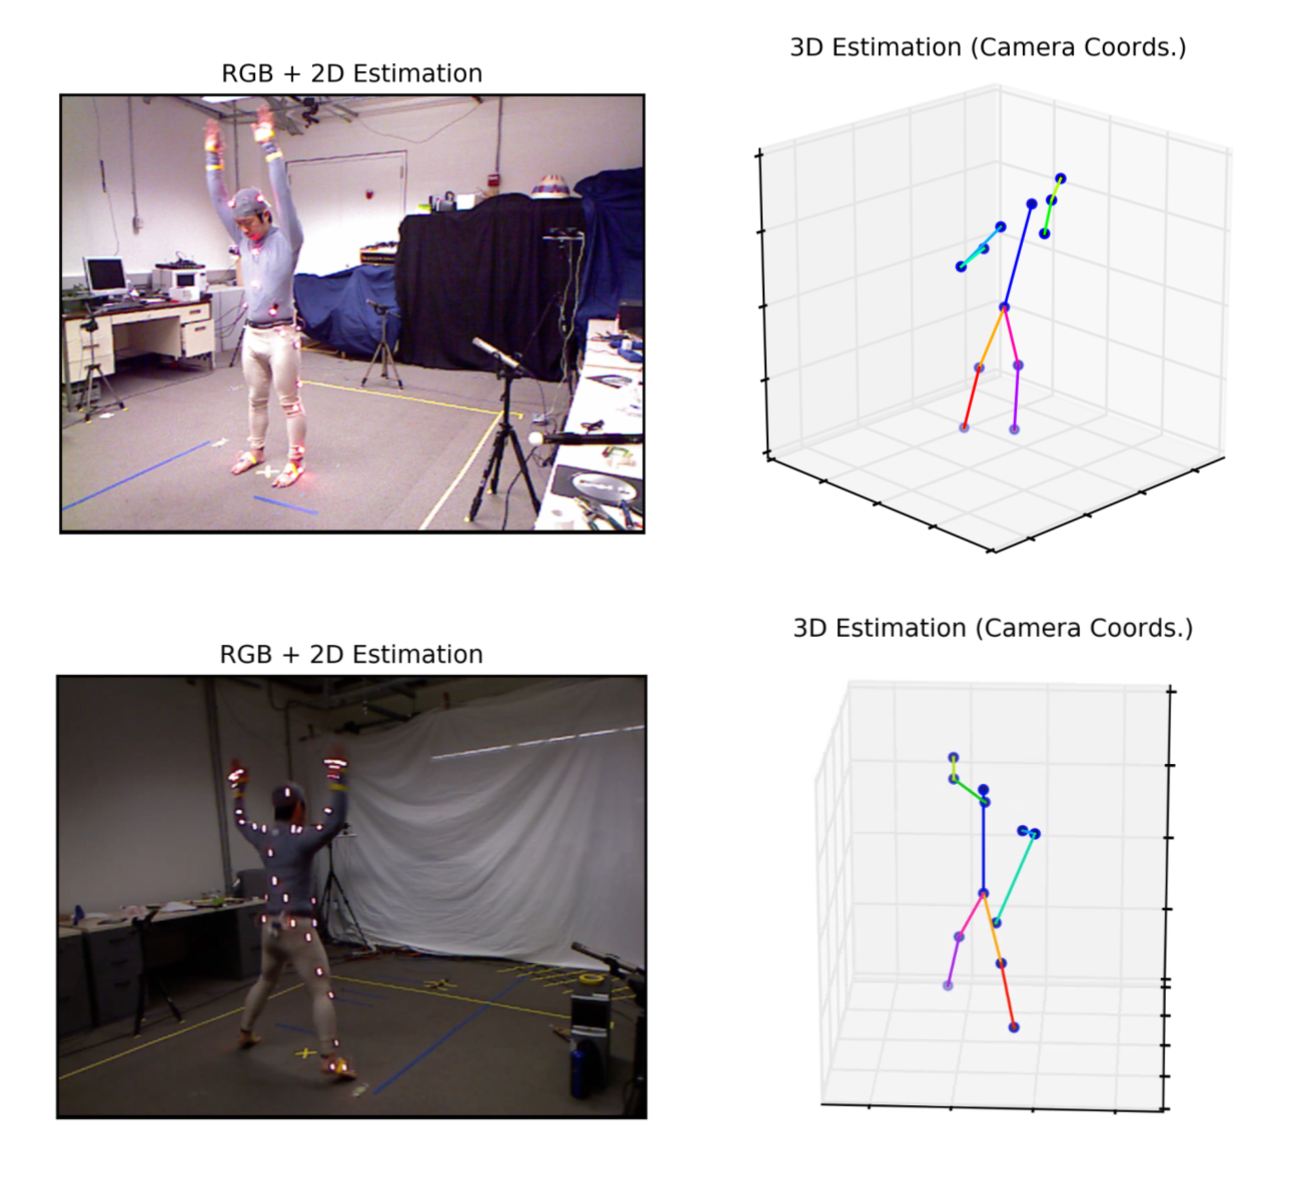
\includegraphics[width=\textwidth]{figures/zimmermann_failed.png} 
        \caption{Outliers found in Zimmermann's estimations.}
        \label{subfig:zimmermann_failed}
    \end{subfigure}
    \begin{subfigure}{0.49\textwidth}\centering
        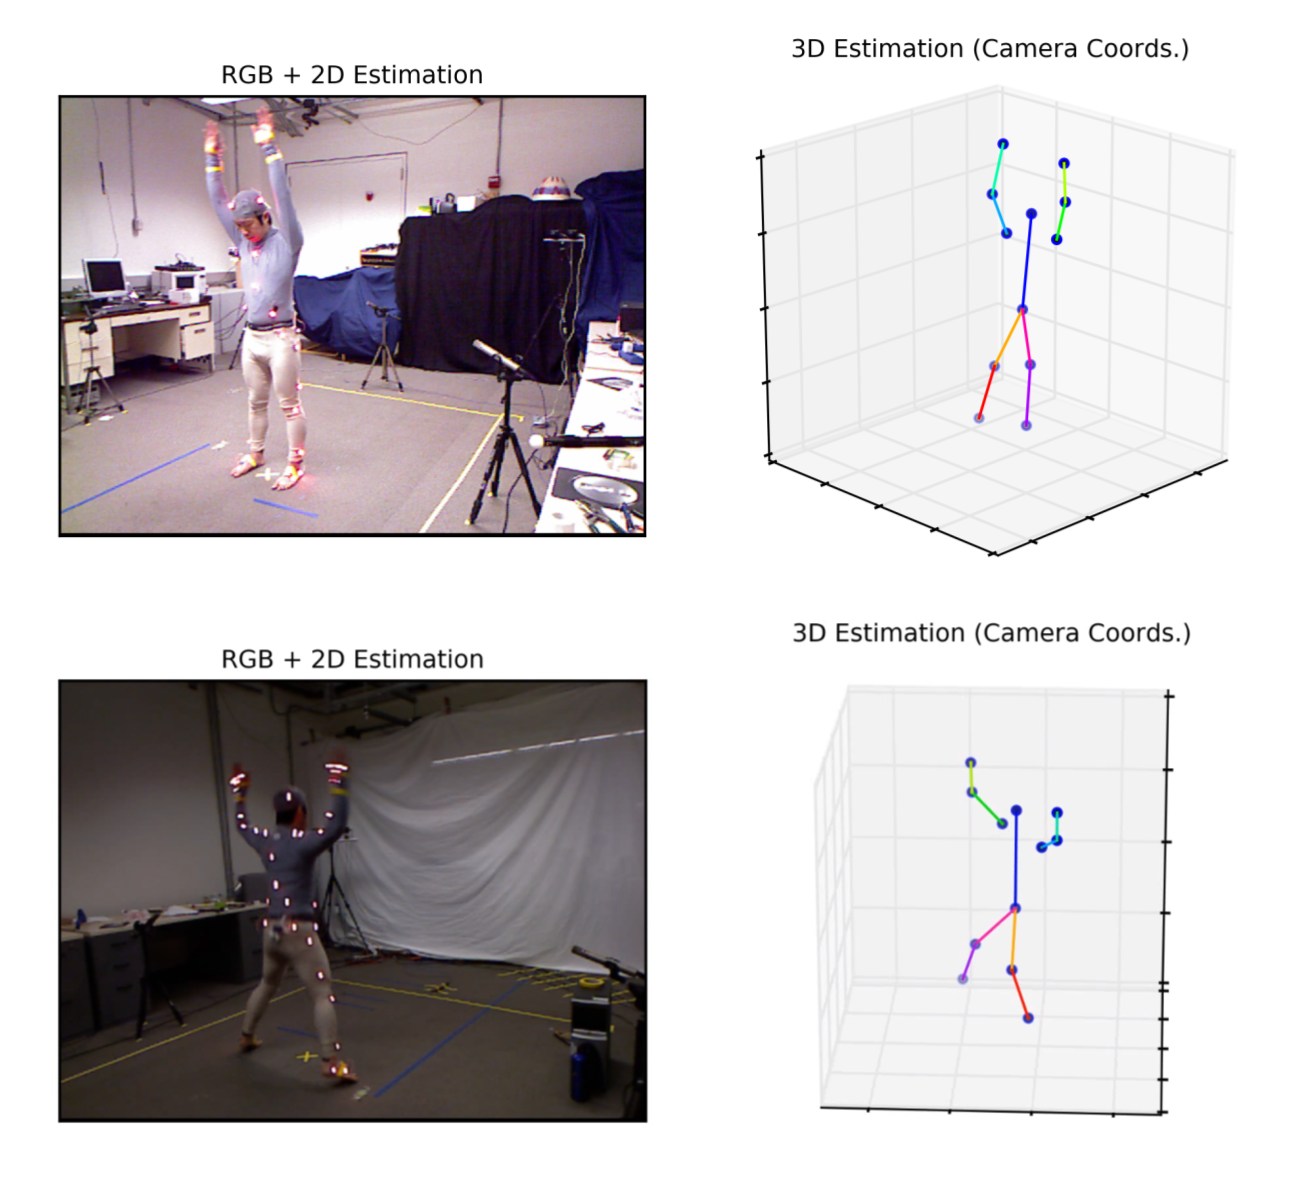
\includegraphics[width=\textwidth]{figures/ours_right.png}
        \caption{Our results for the same frames, using CPMs as 2D estimator.}
        \label{subfig:ours_cpm_right}
    \end{subfigure}
    \caption{Our outlier rejection and filtering mechanisms help alleviate strong deviations like the ones shown in (a). By doing so, even if the overall error in favorable conditions is higher, we get plausible poses consistently (b).}
    \label{fig:zimmermann_failed}
\end{figure}

Regarding the wide difference in terms of pelvis estimation, it is justified by the nature of our method. While Zimmermann's method is trained with labeled 3D joint locations, ours rely on no more than a stream of depth images, from a single point of view, to get the 3D locations from the 2D estimations. With that approach, we cannot \textit{see through} the human body and the only information that we have is the closest point to the camera in the scene when we trace a ray between the sensor and the 2D estimation. Figure~\ref{fig:thickness} exemplifies how this effect might have an impact on our estimations. In that regard, the joint for which this assumption is less precise is the pelvis, as it is placed in a region of the human body thicker than the other keypoints considered, and depending on how the subject is placed on the scene, this thickness changes. In general, our algorithm is more prone to failure if the subject is self-occluded, as it can be see in Figure~\ref{fig:selfocclusion}. A possible solution that might be explored in the future in order to correct this kind of deviations is simply including in our estimations the average thickness of each human body part detected.

\begin{figure}[h]
    \centering
    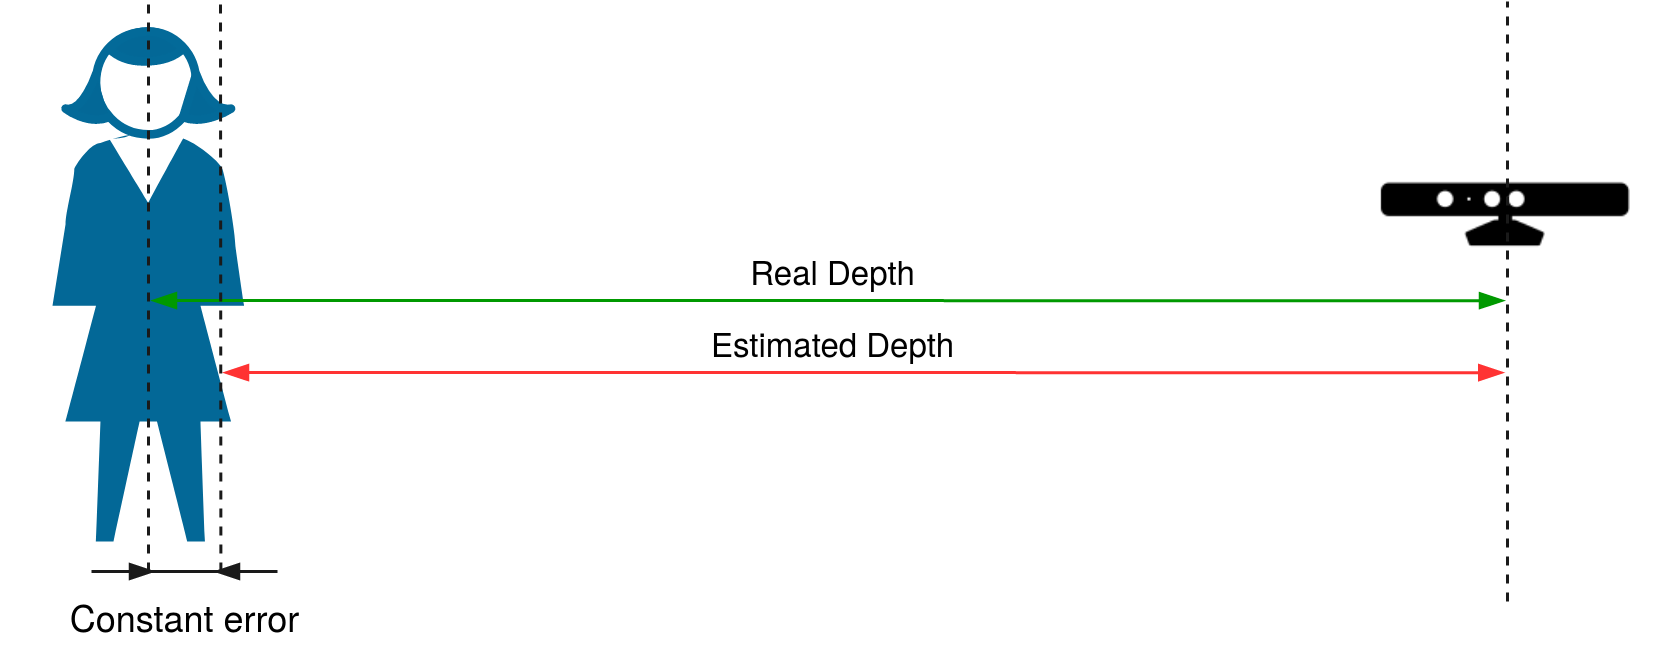
\includegraphics[width=\textwidth]{figures/thickness.png}
    \caption{As our 3D estimations rely on depth images captured from a single point of view and no prior about the human body is imposed, we might commit a constant error when detecting joints that are not labeled close to the body surface.}
    \label{fig:thickness}
\end{figure}

\begin{figure}[h]\centering
    \begin{subfigure}{0.49\textwidth}\centering
        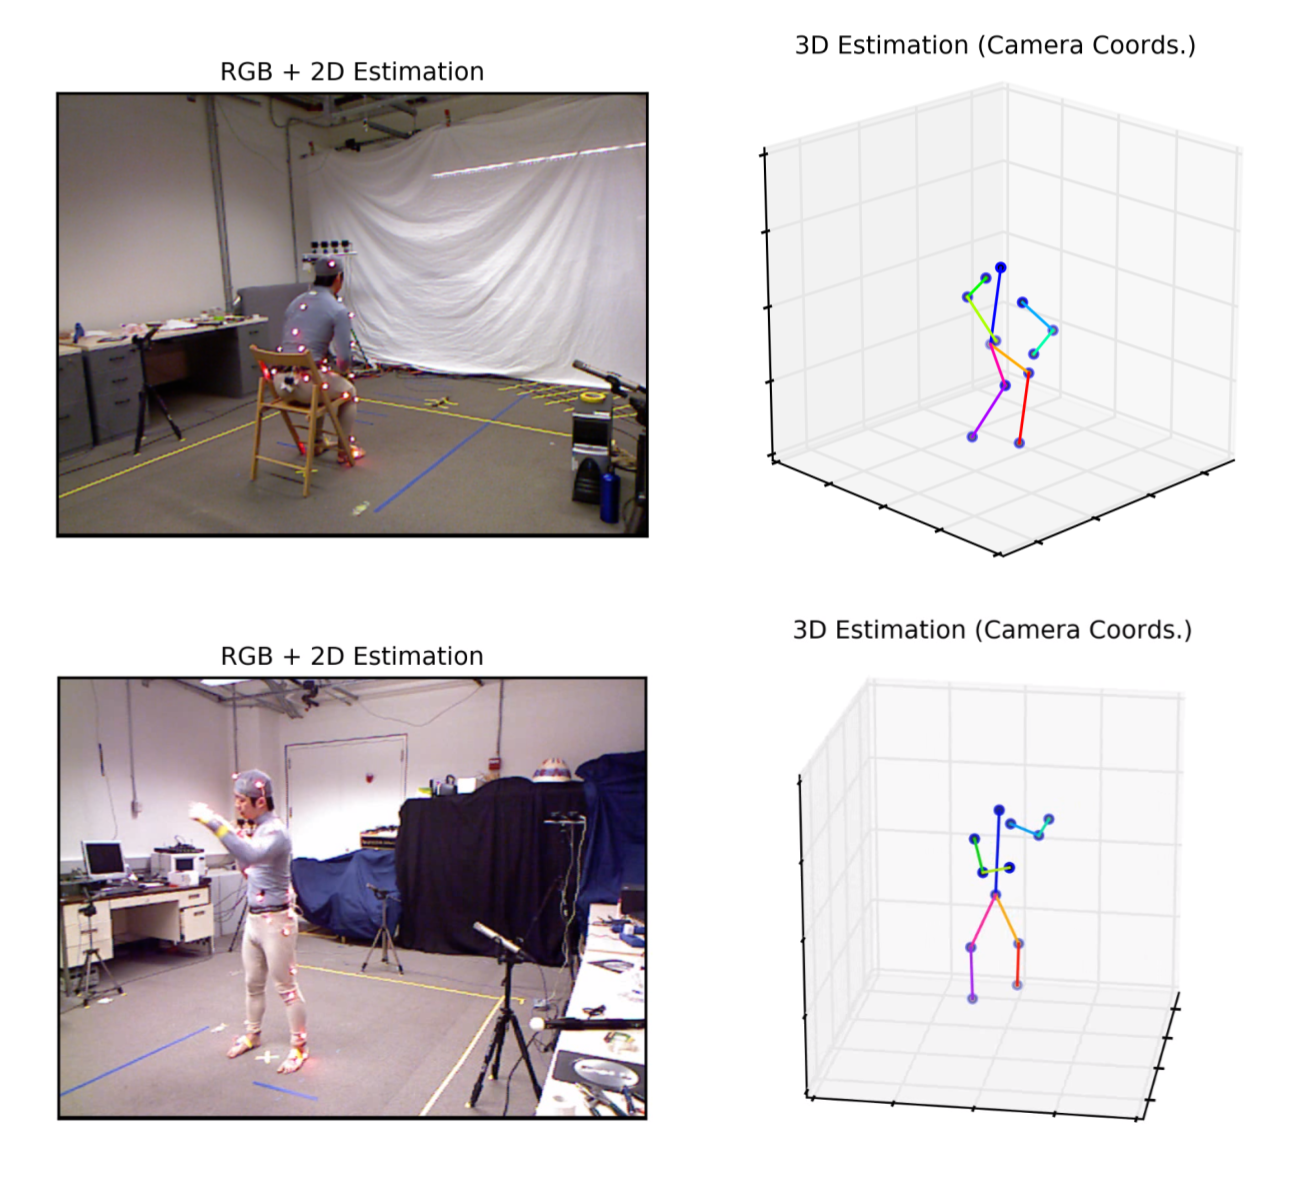
\includegraphics[width=\textwidth]{figures/zimmermann_selfocclusion.png} 
        \caption{Zimmermann's estimation.}
        \label{subfig:zimmermann_selfocclusion}
    \end{subfigure}
    \begin{subfigure}{0.49\textwidth}\centering
        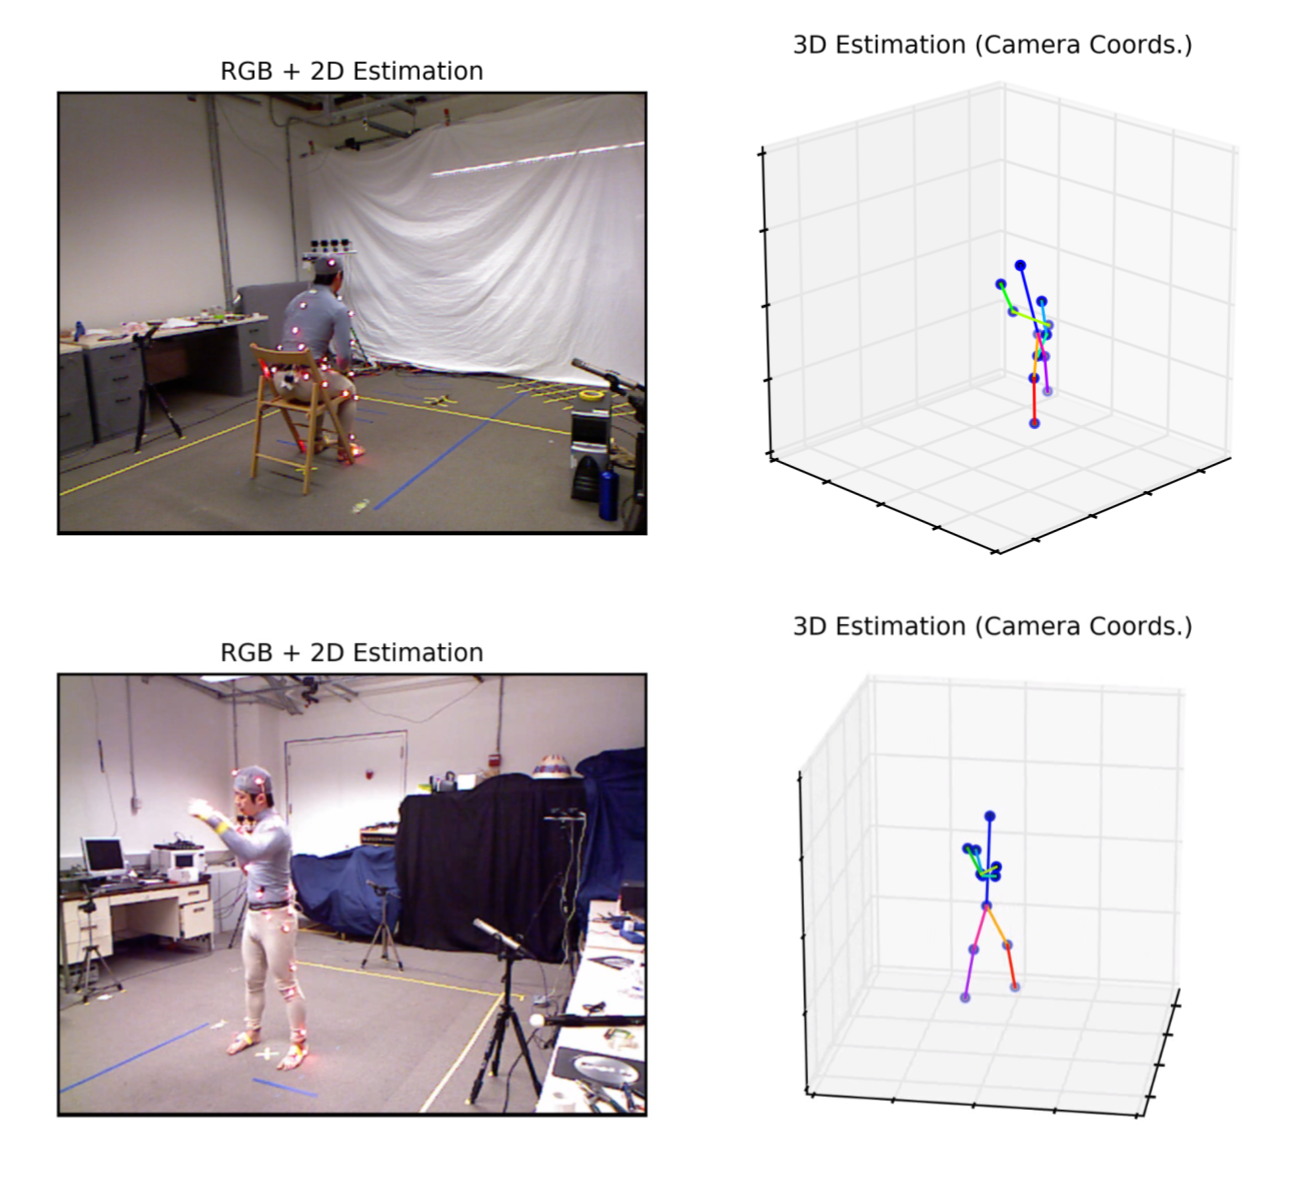
\includegraphics[width=\textwidth]{figures/ours_selfocclusion.png}
        \caption{Our estimation (using CPMs).}
        \label{subfig:ours_selfocclusion}
    \end{subfigure}
    \caption{While Zimmerman's method (a) is able to deal with self-occlusions in the scene, our algorithm (b) relies only on the depth information without any learned prior on the human pose configuration, which causes estimation errors under these circumstances.}
    \label{fig:selfocclusion}
\end{figure}

The same imbalance in \gls{pckh} and \gls{mpjpe} results mentioned in the per joint analysis can be seen when evaluating per action. While our method performs better in three out of eleven actions in terms of \gls{pckh}, it only outperforms Zimmermann's in one of the scenes when evaluating \gls{mpjpe} (see Table~\ref{tab:mpjpe_action} and Table~\ref{tab:pckh_3d_action}).

\begin{table}[!ht]  
  \centering
  \resizebox{\textwidth}{!}{\begin{tabular}{l||oorobbbrggg|c}
    \hline
    & a01 & a02 & a03 & a04 & a05 & a06 & a07 & a08 & a09 & a10 & a11 & TOTAL \\
    \hline
    \glspl{cpm} & 124.3 & 123.8 & \textbf{159.7} & 156.1 & 117.5 & 116.9 & 139.2 & 135.8 & 173.6 & 178.0 & 166.1 & 144.1 \\
    \gls{sh} & 123.7 & 119.8 & 163.1 & 158.1 & 122.6 & 128.9 & 141.8 & 146.4 & 179.7 & 186.5 & 171.6 & 148.7 \\
    \glspl{cp} & 138.6 & 150.5 & 181.0 & 172.5 & 146.6 & 146.4 & 155.2 & 171.0 & 185.9 & 206.0 & 175.7 & 164.8 \\
    Zimm. & \textbf{105.8} & \textbf{114.5} & 179.4 & \textbf{120.6} & \textbf{115.9} & \textbf{102.7} & \textbf{116.0} & \textbf{118.0} & \textbf{137.4} & \textbf{157.6} & \textbf{133.7} & \textbf{128.1} \\
    \hline
  \end{tabular}}
  \caption{Quantitative 3D pose estimation results on BMHAD per action, using as figure of merit MPJPE (mm). Values in bold correspond to the best results achieved for each category. Columns are colored following the convention established in Section~\ref{sec:benchmark_dataset}.}
  \label{tab:mpjpe_action}
\end{table}

\begin{table}[!ht]  
  \centering
  \resizebox{\textwidth}{!}{\begin{tabular}{l||oorobbbrggg|c}
    \hline
    & a01 & a02 & a03 & a04 & a05 & a06 & a07 & a08 & a09 & a10 & a11 & TOTAL \\
    \hline
    \glspl{cpm} & 89.48 & 91.16 & \textbf{71.25} & 78.15 & \textbf{92.94} & 91.57 & 84.67 & 84.73 & 70.54 & 67.69 & 73.03 & 80.23 \\
    \gls{sh} & 89.39 & \textbf{91.99} & 65.69 & 77.54 & 92.12 & 90.08 & 83.33 & 82.10 & 70.36 & 67.32 & 72.42 & 78.70 \\
    \glspl{cp} & 86.29 & 85.18 & 60.46 & 75.21 & 85.60 & 84.45 & 81.59 & 79.21 & 69.00 & 64.52 & 71.12 & 74.88 \\
    Zimm. & \textbf{94.15} & 90.52 & 55.91 & \textbf{87.83} & 89.25 & \textbf{93.07} & \textbf{89.06} & \textbf{88.57} & \textbf{81.97} & \textbf{73.02} & \textbf{80.78} & \textbf{81.55} \\
    \hline
  \end{tabular}}
  \caption{Quantitative 3D pose estimation results on BMHAD per action, using as figure of merit PCKh~3D~@~1~(\%). Values in bold correspond to the best results achieved for each category. Columns are colored following the convention established in Section~\ref{sec:benchmark_dataset}.}
  \label{tab:pckh_3d_action}
\end{table}

If we compare results after grouping the actions in terms of dynamics and occlusion, it is shown that our method performs better in the most challenging scenarios, \ie very dynamic actions with occluded joints. This observation holds true for both \gls{pckh} in Table~\ref{tab:pckh_3d_action_type} and \gls{mpjpe} in Table~\ref{tab:mpjpe_action_type}. These differences can be caused again by our outlier rejection and Kalman filtering stages, which reduce the number of greatly deviated estimations in an explicit manner. Meanwhile, Zimmermann's method does not apply any post-processing on the yielded estimations and so great errors might appear when, for instance, a joint gets out of view or the subject is moving too fast. 

\begin{table}[!ht]  
  \centering
  \resizebox{\textwidth}{!}{\begin{tabular}{l||ro|gb}
    \hline
    & \multicolumn{2}{c|}{High Dynamics} & \multicolumn{2}{c}{Low Dynamics} \\
    \cline{2-5}
    & Heavily Occluded & Slightly Occluded & Heavily Occluded & Slightly Occluded \\
    \hline
    \glspl{cpm} & \textbf{77.99} & 86.26 & 70.42 & 89.73 \\
    \gls{sh} & 73.90 & 86.31 & 70.03 & 88.51 \\
    \glspl{cp} & 69.83 & 82.22 & 68.21 & 83.88 \\
    Zimm. & 72.24 & \textbf{90.83} & \textbf{78.59} & \textbf{90.46} \\
    \hline
  \end{tabular}}
  \caption{Quantitative 3D pose estimation results on BMHAD per action type, using as figure of merit PCKh~3D~@~1~(\%). Values in bold correspond to the best results achieved for each category. Columns are colored following the convention established in Section~\ref{sec:benchmark_dataset}.}
  \label{tab:pckh_3d_action_type}
\end{table}

\begin{table}[!ht]  
  \centering
  \resizebox{\textwidth}{!}{\begin{tabular}{l||ro|gb}
    \hline
    & \multicolumn{2}{c|}{High Dynamics} & \multicolumn{2}{c}{Low Dynamics} \\
    \cline{2-5}
    & Heavily Occluded & Slightly Occluded & Heavily Occluded & Slightly Occluded \\
    \hline
    \glspl{cpm} & \textbf{147.8} & 134.7 & 172.6 & 124.5 \\
    \gls{sh} & 154.8 & 133.9 & 179.3 & 131.1 \\
    \glspl{cp} & 176.0 & 153.9 & 189.2 & 149.4 \\
    Zimm. & 148.7 & \textbf{113.6} & \textbf{142.9} & \textbf{111.6} \\
    \hline
  \end{tabular}}
  \caption{Quantitative 3D pose estimation results on BMHAD per action type, using as figure of merit MPJPE (mm). Values in bold correspond to the best results achieved for each category. Columns are colored following the convention established in Section~\ref{sec:benchmark_dataset}.}
  \label{tab:mpjpe_action_type}
\end{table}

An interesting lesson from the results we have just discussed is that our method for filtering 3D estimations could easily be plugged in after another 3D human pose estimation method such as Zimmermann's, further improving their results. By doing so, we would increase the computational cost, which is a major requirement in this work, but whether this could be a reasonable solution or not depends on the application.

\section{Computational burden}\label{sec:computational_burden}
Besides achieving very competitive quantitative results when compared with the \gls{sota} method introduced by Zimmermann \etal\cite{Zimmermann2018-sn}, we keep the computational costs as low as possible by using very lightweight algorithms for the 2D to 3D augmentation of the estimated coordinates. In Table~\ref{tab:computational_burden}, a comparison of the computational burden associated with each evaluated method in previous sections is presented. All the tests have been performed after evaluating 2108 frames of 10 different scenes extracted from \gls{bmhad}, using a PC with the following specifications:

\begin{itemize}
    \item \textbf{RAM memory}: 12Gb.
    \item \textbf{GPU}: Nvidia GeForce GTX 1050.
    \item \textbf{CPU}: Intel Core i7-7700HQ @ 2.80GHz
\end{itemize}

\begin{table}[!ht]  
  \centering
  \resizebox{\textwidth}{!}{\begin{tabular}{l||cccc|c}
    \hline
    & \glspl{cpm} & \gls{sh} & \glspl{cp} & Zimm. & Our 2D to 3D registration module alone\\
    \hline
    \gls{fps} & 8.11 & \textbf{16.07} & 10.64 & 2.22 & \textbf{99.76}\\
    \hline
  \end{tabular}}
  \caption{Computational cost of each method, measured as the average number of frames per second.}
  \label{tab:computational_burden}
\end{table}

As it can be seen, our methods perform with much higher framerates, which facilitates their inclusion in robotic systems as embedded software. For instance, our method is around four times faster than Zimmermann's when using \glspl{cpm} as 2D estimator, and more than seven times faster when using \gls{sh}. When measuring the time that it takes to carry out the 2D to 3D step, without taking into account the 2D estimation process, our algorithm only adds 0.01s to the total computation time for a single frame.

It is also worth mentioning that the computational burden can be further reduced depending on the boxsize of the input image. Depending on the accuracy required by the application, an optimal trade-off between the quality of the estimation and the computational cost may be explored.

\section{Qualitative evaluation: real-time demo}\label{sec:demo}
We have already discussed how our method compares with the \gls{sota}, both in terms of accuracy and computational burden. Our approach cannot outperform the most recent works in the literature in 3D human pose estimation, but it is competitive and much faster. However, the tests carried out have not assessed its performance with more common scenes \emph{in the wild}. For that purpose, we have developed a real-time demo that works in an \emph{off-the-shelf} computer with a commercial RGBD sensor. The set-up used and the system designed for that demo are presented in this section, along with a discussion about the obtained results.

In Figure~\ref{fig:setup}, the simple set-up built for this demo is presented. Our demo has been run on a PC with the specifications described in Section~\ref{tab:computational_burden}. This PC is equipped with an Nvidia GPU~\cite{nvidia}, which allows the 2D estimator to make use of the CUDA parallel computing platform~\cite{nickolls2008scalable} for accelerating the inference of the human poses. The RGBD sensor used for the demo is an Asus Xtion PRO LIVE~\cite{xtion}. This camera captures RGBD video sequences at 30\gls{fps} with a resolution of 640x480 pixels and a working distance that ranges between 0.5 and 3.5 meters. It relies on an infrared sensor and structured light projected on the scene for estimating depth.

\begin{figure}[h]\centering
    \begin{subfigure}{\textwidth}\centering
        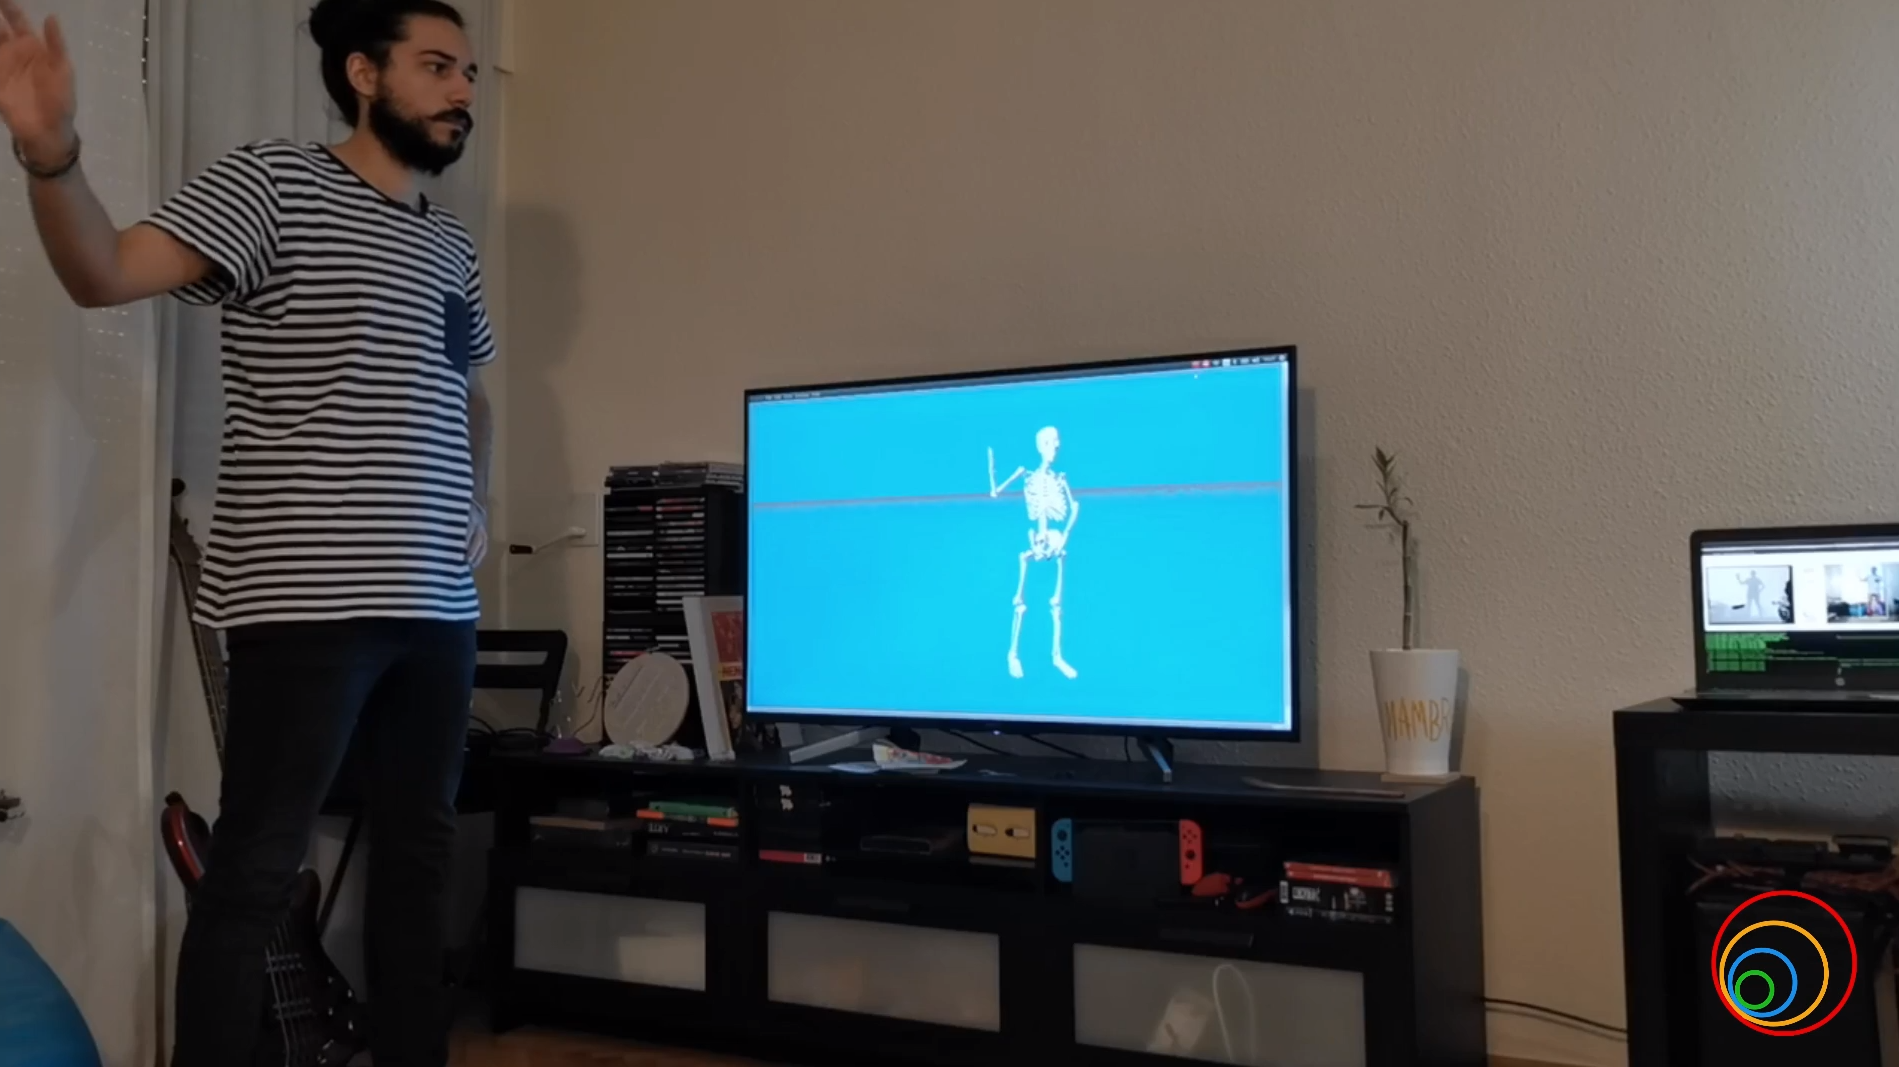
\includegraphics[width=\textwidth]{figures/real_setup.png} 
        \caption{Image from the real set-up.}
        \label{subfig:real_setup}
    \end{subfigure}
    \begin{subfigure}{\textwidth}\centering
        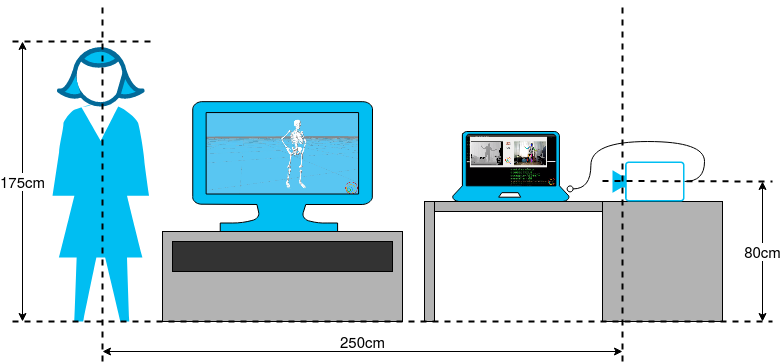
\includegraphics[width=\textwidth]{figures/setup.png}
        \caption{Simplified diagram with relevant distances.}
        \label{subfig:simple_setup}
    \end{subfigure}
    \caption{Diagram of the set-up used for the real-time demo.}
    \label{fig:setup}
\end{figure}

Regarding the software used for the demo, our system employs ROS~\cite{ros} for PC-camera communication. In particular, we have used the \emph{openni2} node~\cite{openni}, which allows depth and RGBD image registration and distortion correction, based on our camera calibration data. Our demo application has been entirely developed in \emph{Python} in a threaded manner. A thread is in charge of receiving and serving the color and depth images provided by the ROS node. Another thread updates a GUI that shows in real time these images and the result of the 2D pose estimation. Last but not least, a third thread is in charge of estimating the 2D poses and, from these, generating the final 3D estimations as described in Section~\ref{sec:3d_estimation}. These 3D estimations can then be inspected in real-time thanks to the 3D visualizer gently shared by Roberto Pérez~\cite{perez_gonzalez_2019}. This visualizer has been built as a desktop app developed with Electron~\cite{electron}. It is important to note that, for this demo, we have used \glspl{cpm} as 2D estimator. In order to further improve the framerate we have used a boxsize of 256x256, which yields good enough results. A complete diagram of the developed software can be seen in Figure~\ref{fig:sw}. The  developed application is publicly available and hosted in \emph{GitHub}~\footnote{\url{https://github.com/RoboticsLabURJC/2017-tfm-david-pascual/}}.% the figure must include screenshots from the GUIs

\begin{figure}[h]
    \centering
    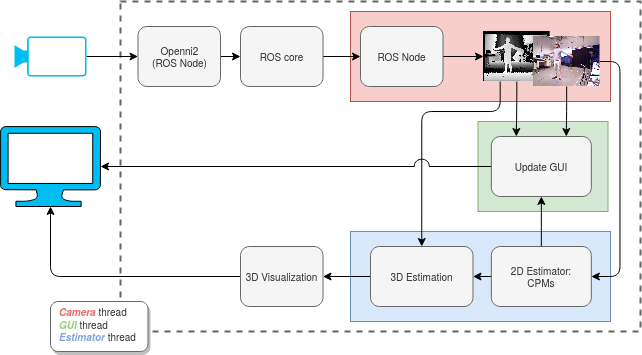
\includegraphics[width=\textwidth]{figures/sw.png}
    \caption{Overview of the application developed.}
    \label{fig:sw}
\end{figure}

Results for this demo are in Figure~\ref{fig:demo_result}. The application runs fluently in real-time and, in general, achieves good results for the tested poses. It is worth mentioning that we identify failures in certain situations, \eg when the subject is too close to the camera or stands sidewards, which increases the number of occluded joints. Such cases can be seen in Figure~\ref{fig:demo_failures}. A complete video showcasing the described demo is publicly available on \emph{YouTube}~\footnote{\url{https://www.youtube.com/watch?v=W3XirsadmNg}}.

\begin{figure}[h]\centering
    \begin{subfigure}{\textwidth}\centering
        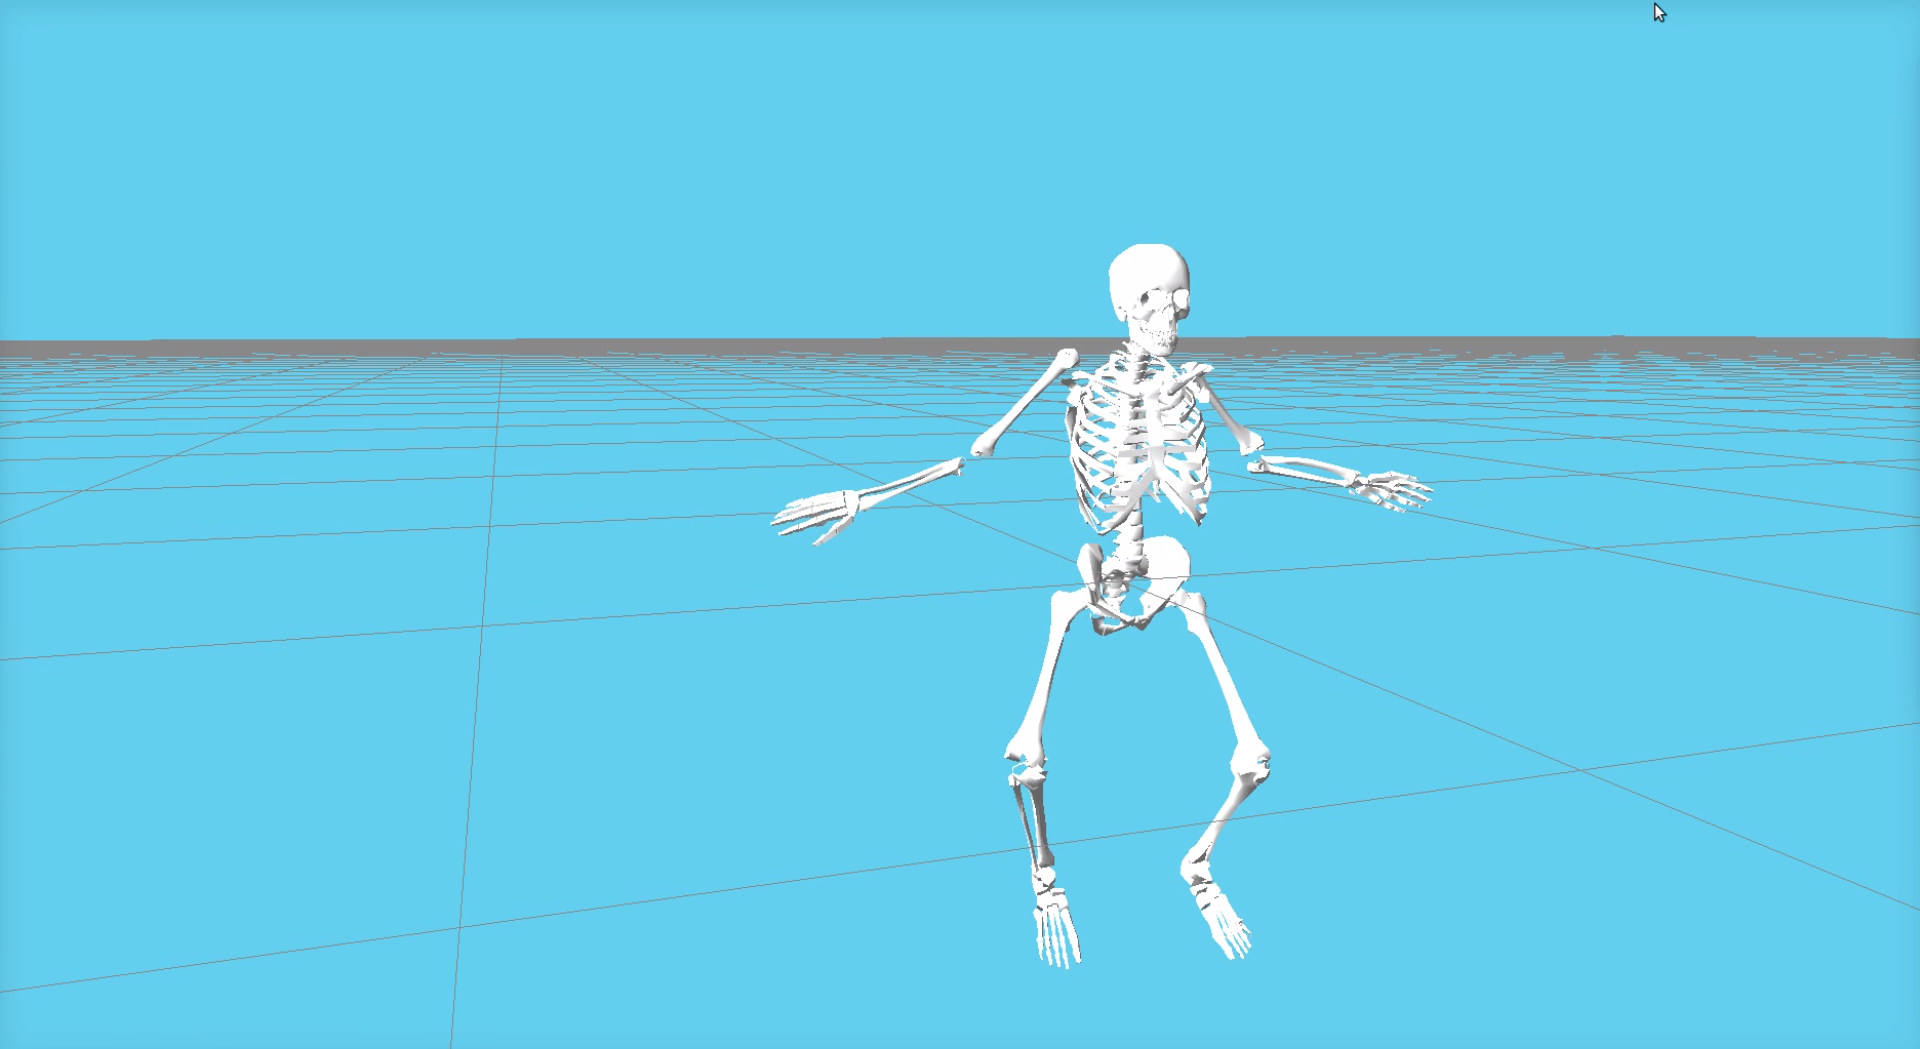
\includegraphics[width=\textwidth]{figures/gui_3d.png} 
        \caption{3D estimation results.}
        \label{subfig:gui_3d}
    \end{subfigure}
    \begin{subfigure}{\textwidth}\centering
        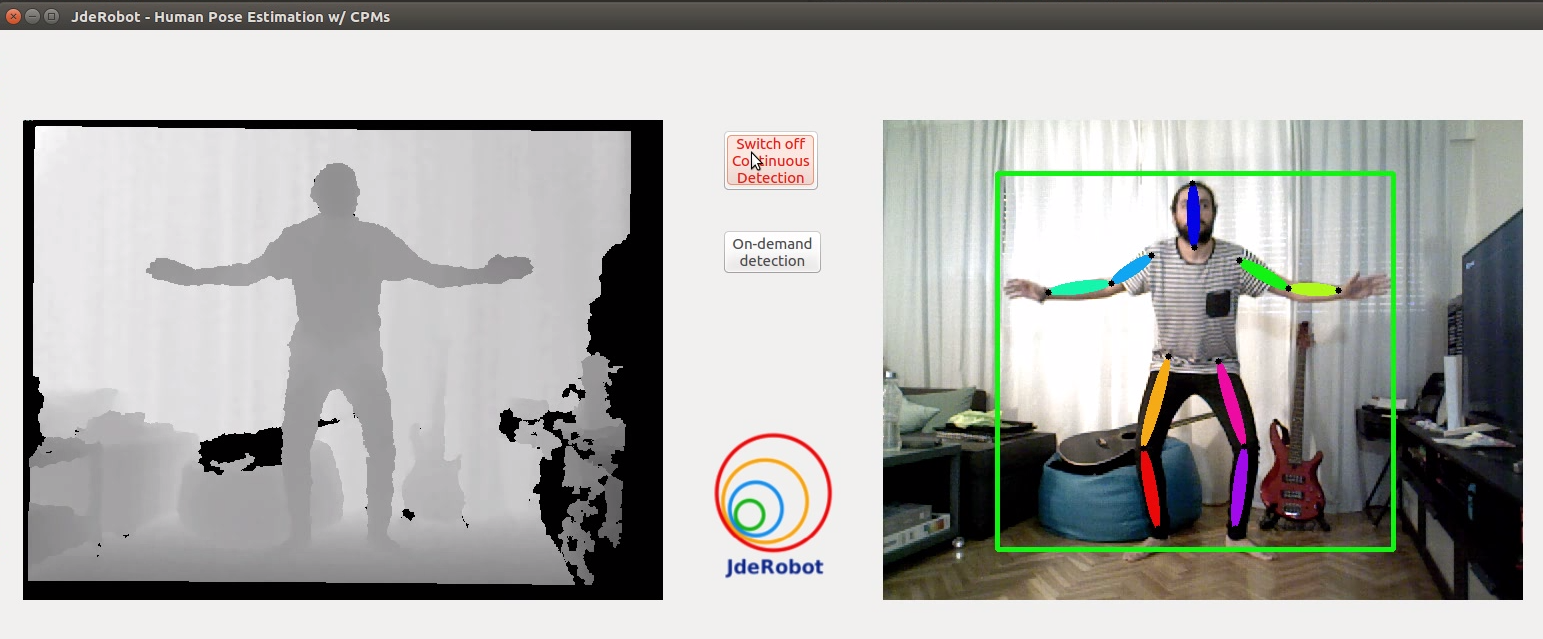
\includegraphics[width=\textwidth]{figures/gui_2d.png}
        \caption{2D estimation results.}
        \label{subfig:gui_2d}
    \end{subfigure}
    \caption{Real-time results as presented by our application for (a) 3D pose estimation and (b) 2D estimation.}
    \label{fig:demo_result}
\end{figure}

\begin{figure}[h]\centering
    \begin{subfigure}{0.49\textwidth}\centering
        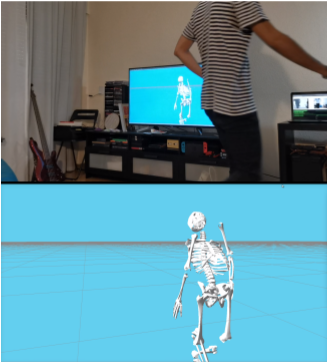
\includegraphics[width=0.99\textwidth]{figures/too_close.png} 
        \caption{Estimation fails due to subject proximity.}
        \label{subfig:too_close}
    \end{subfigure}
    \begin{subfigure}{0.49\textwidth}\centering
        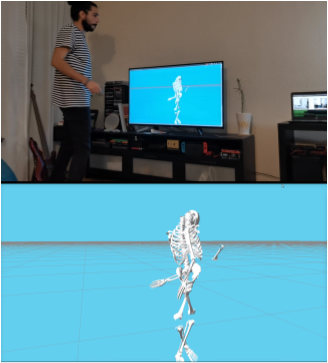
\includegraphics[width=0.99\textwidth]{figures/occlusion.png}
        \caption{Estimation in auto-occlusion.}
        \label{subfig:occlusion}
    \end{subfigure}
    \caption{Our algorithm might fail in challenging scenarios, such as (a) the subject being too close to the camera or (b) self-occlusions.}
    \label{fig:demo_failures}
\end{figure}
\lhead[]{CHAPTER \thechapter. CONCLUSIONS}
\chapter{Conclusions}\label{sec:conclusions}

%%%%%%%%%%%%%%% Bibliography %%%%%%%%%%%%%%%
\addcontentsline{toc}{chapter}{Bibliography}
\printbibliography


\end{document}